\section{Background estimation}
\label{bg}
\fxnote{add intro blurb?}
\subsection{Background sources}
\label{bg_sources}
The vast majority of leptons from SM processes are prompt. There are, however, a few notable processes that produce leptons with large \ad values that may pass our selection: (1) leptons from prompt decays whose \ad is poorly measured ("mismeasurements"), (2) leptons from  decays of tau leptons ("taus"), and (3) leptons from decays of B or D mesons ("heavy flavor"). Note that the leptons from these processes generally do not share a common displaced vertex. We perform several cross checks to ensure that processes in which leptons share a common displaced vertex do not contribute significantly in the signal regions (SRs). Section~\ref{additional_bg_checks} presents several additional studies that confirm that the SR contribution of leptons from material interactions, cosmic rays, and SM hadrons are either negligible or already accounted for by the background estimation procedure.

The \ad distributions of leptons from the three main background sources vary according to lepton flavor and parent particle. Tau leptons have a lifetime of \SI{87}{\um}, B mesons have a lifetime around \SI{500}{\um}, and D mesons have a lifetime of around \SI{100}{\um}, so leptons from taus will generally have smaller \ad values than leptons from heavy flavor. Furthermore, mismeasurements are more common for electrons than for muons due to the superior muon $d_0$ resolution. Figure~\ref{ttbar_d0_behavior}, which shows the relative contribution of each source of leptons as a function of \ad in simulated \ttbar events that pass the \Pe\Pgm\ channel preselection, shows how mismeasurements dominate at all \ad values for electrons while taus and heavy-flavor contribute meaningfully for muons with $\ad\gtrsim\SI{100}{\um}$.\fxnote{rewrite this paragraph to properly introduce the correlation concept}

\begin{figure}
\centering
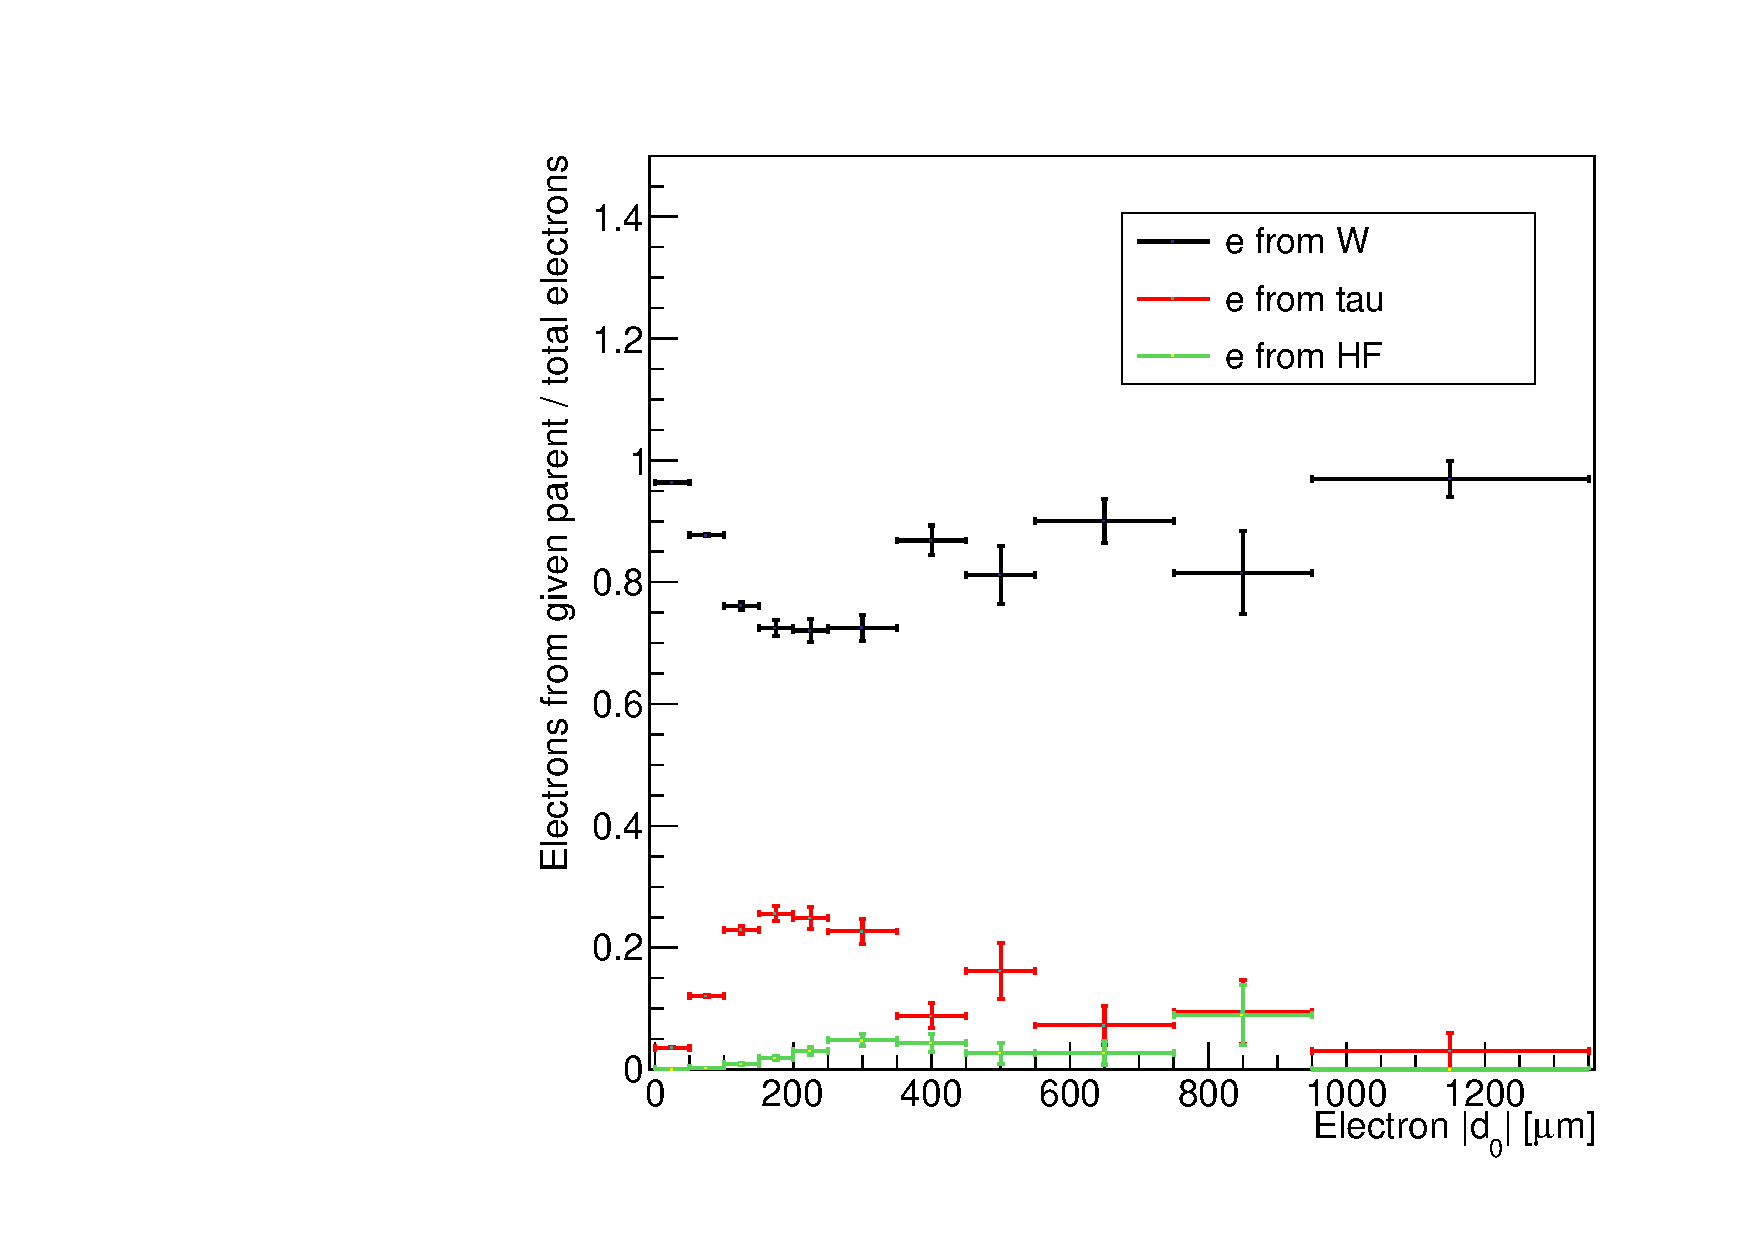
\includegraphics[width=0.49\textwidth]{figures/bg/emu_tt_electronAbsD0_1000um_variableBins_coarse_ratios.pdf}
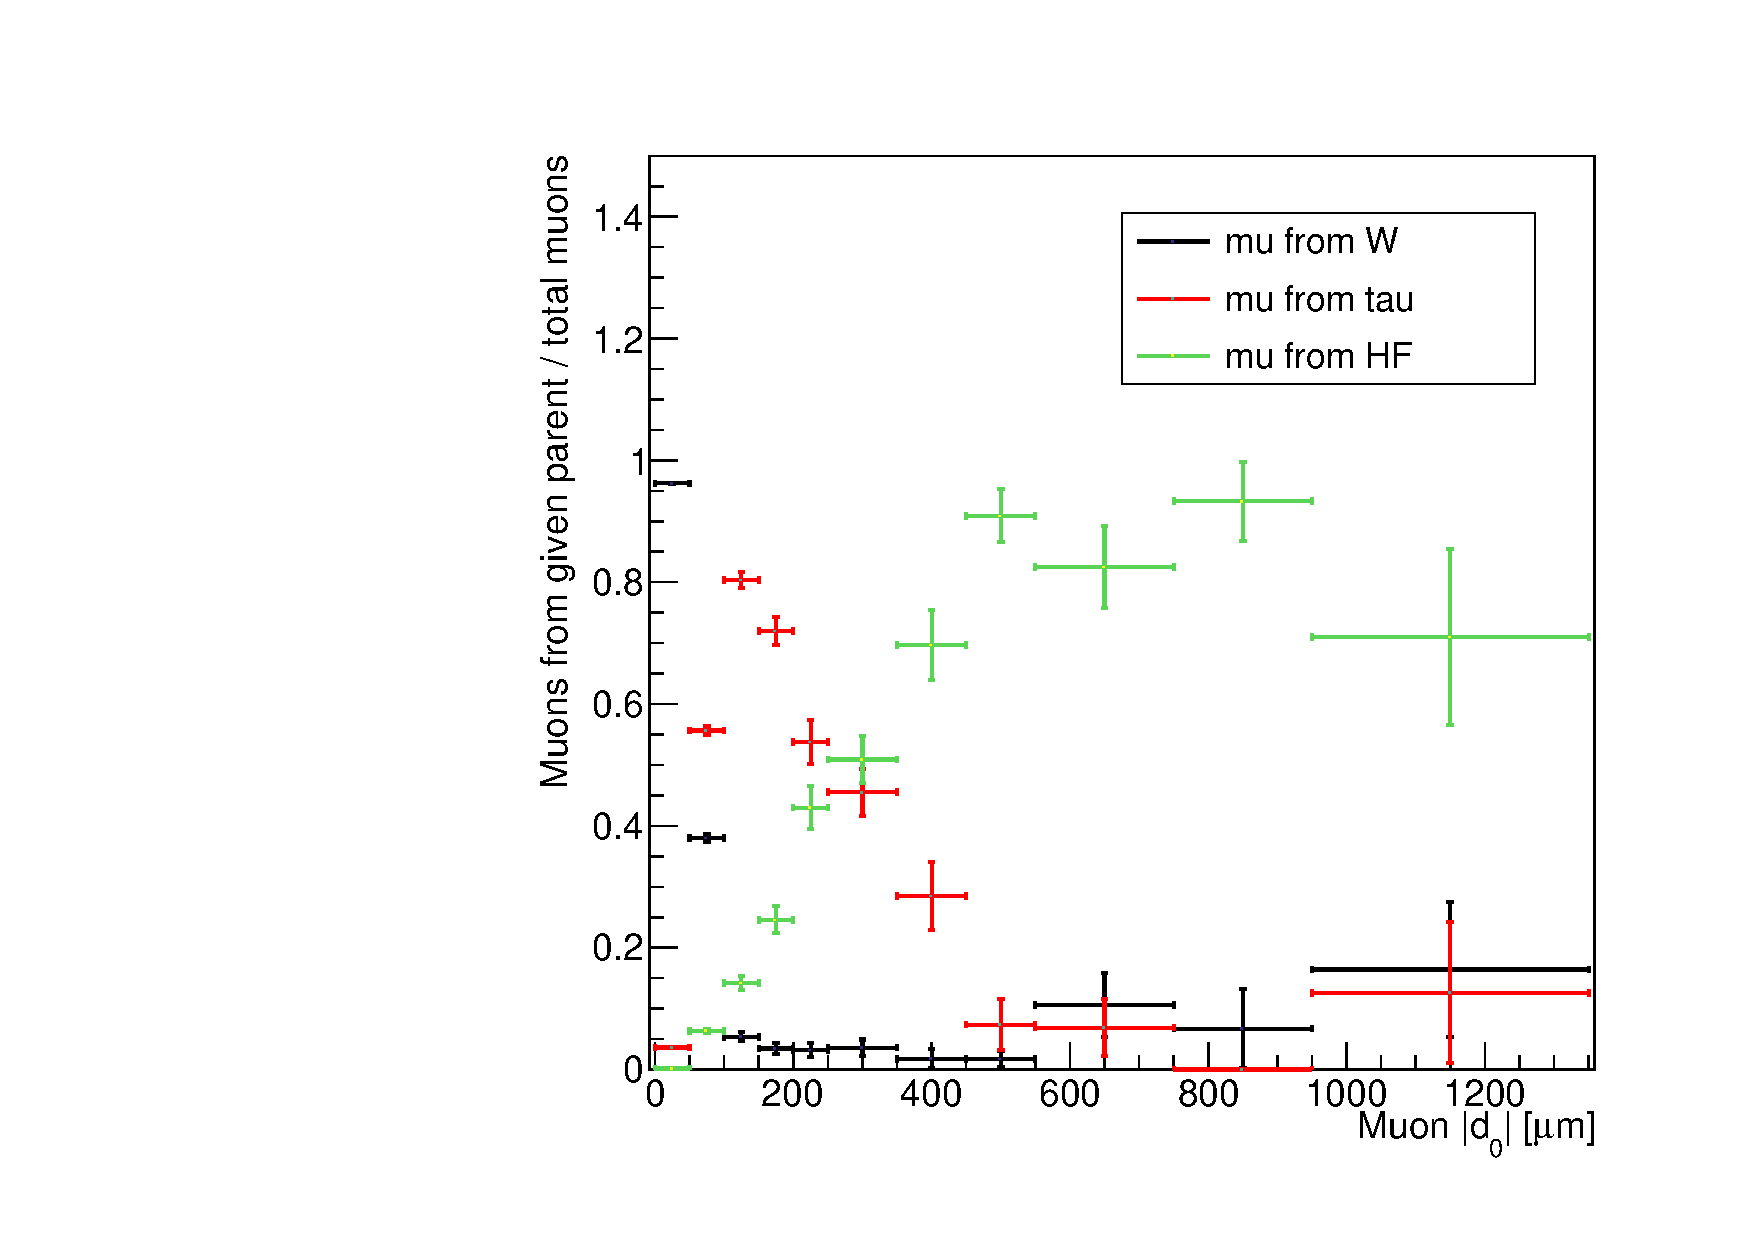
\includegraphics[width=0.49\textwidth]{figures/bg/emu_tt_muonAbsD0_1000um_variableBins_coarse_ratios.pdf}
\caption{The fraction of electrons (left) and muons (right) from different parents as a function of lepton \ad, for simulated \ttbar events that pass the 2018 $\Pe\Pgm$ channel preselection. In \ttbar events, the vast majority of leptons whose parent is a $\PW$ boson are produced in a prompt decay.}
\label{ttbar_d0_behavior}
\end{figure}

\fxnote{rewrite this section to first introduce correlation concept, then single out taus and show mumu dy plot; don't forget to mention 2016 vs 2017--2018}
In the \Pgm\Pgm\ channel, it is worth examining which long-lived SM parents will contribute to \ad-\ad correlation. The correlation specifically comes from DY-type processes in which the parentage is correlated between muons. Figure~\ref{dy_d0_behavior}, which shows the fraction of muons from different background sources in DY simulation, indicates that tau lepton decays are the main source of muons that may be correlated in this way, and that the heavy-flavor contribution is negligible. This is reasonable because while tau leptons and heavy-flavor mesons both produce displaced muons, the isolation criteria rejects the vast majority of muons from heavy-flavor mesons.  Muons from tau leptons contribute significantly from about \num{100} to \SI{500}{\um}, so we expect the most significant \ad-\ad correlation to appear in this range and peak around \SI{200}{\um}. Furthermore, the correlation will be most pronounced in the regions where the \ad measurements are the best.

\begin{figure}
\centering
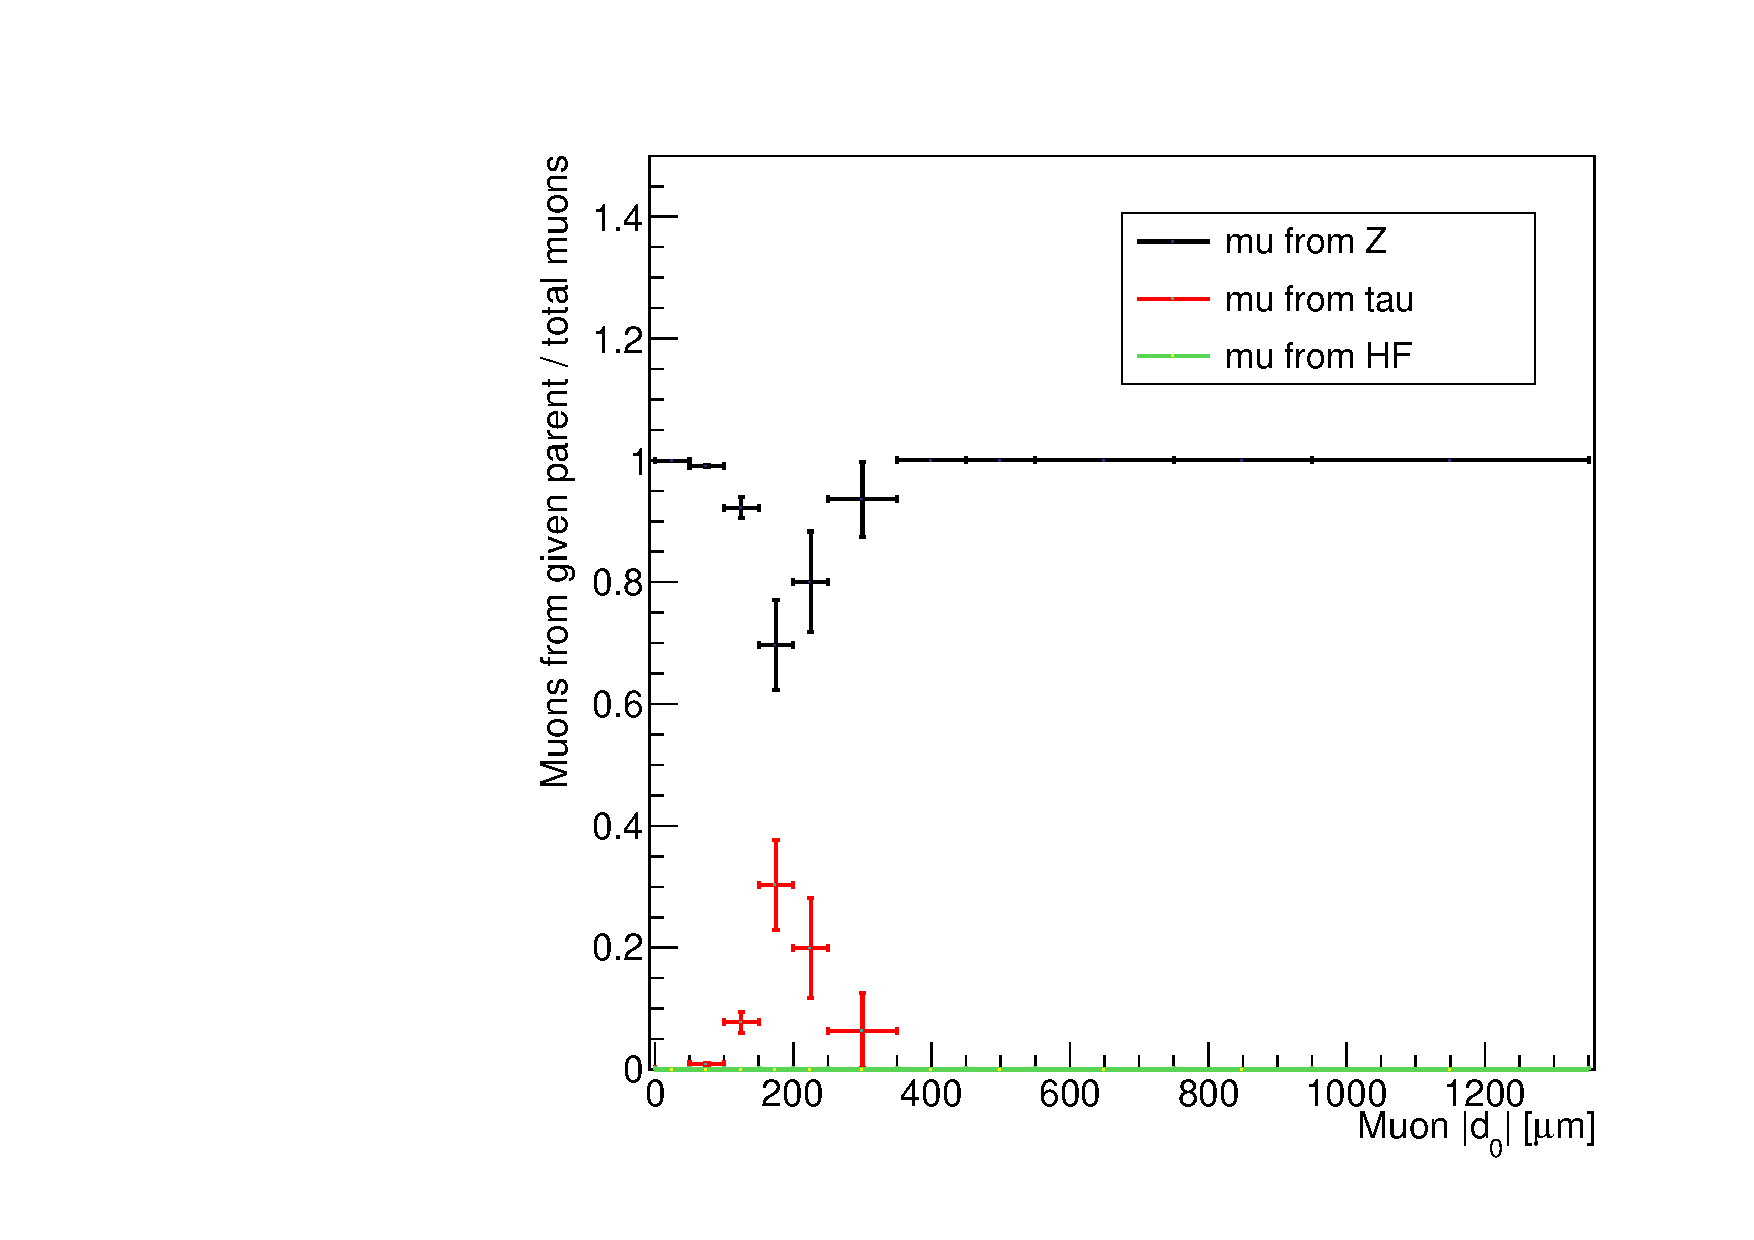
\includegraphics[scale=0.35]{figures/bg/mumu_DY_muonAbsD0_1000um_variableBins_coarse_ratios.pdf}
\caption{The fraction of muons from different parents as a function of muon \ad, for simulated DY events that pass the 2018 $\Pgm\Pgm$ channel preselection and the additional constraint that the leading and subleading muon both come from the same type of parent particle.}
\label{dy_d0_behavior}
\end{figure}

\subsection{Data-driven ABCD method}
\label{abcd}
We estimate the SR background yields with a data-driven method in which the lepton \ad distributions serve as composite models of all background processes. Specifically, we employ an ABCD method using the \ad of two leptons. We label the two \ad values in each channel as \ada and \adb, which correspond to the leading $\Pe$ and leading $\Pgm$ in the \Pe\Pgm\ channel, the leading and subleading $\Pe$ in the \Pe\Pe\ channel, and the leading and subleading $\Pgm$ in the \Pgm\Pgm\ channel. As a first step, we categorize the events that pass the preselection criteria into four regions (A, B, C, and D) of the \ada-\adb plane, as shown in Fig.~\ref{abcd_regions}.

\begin{figure}[hbtp]
\centering
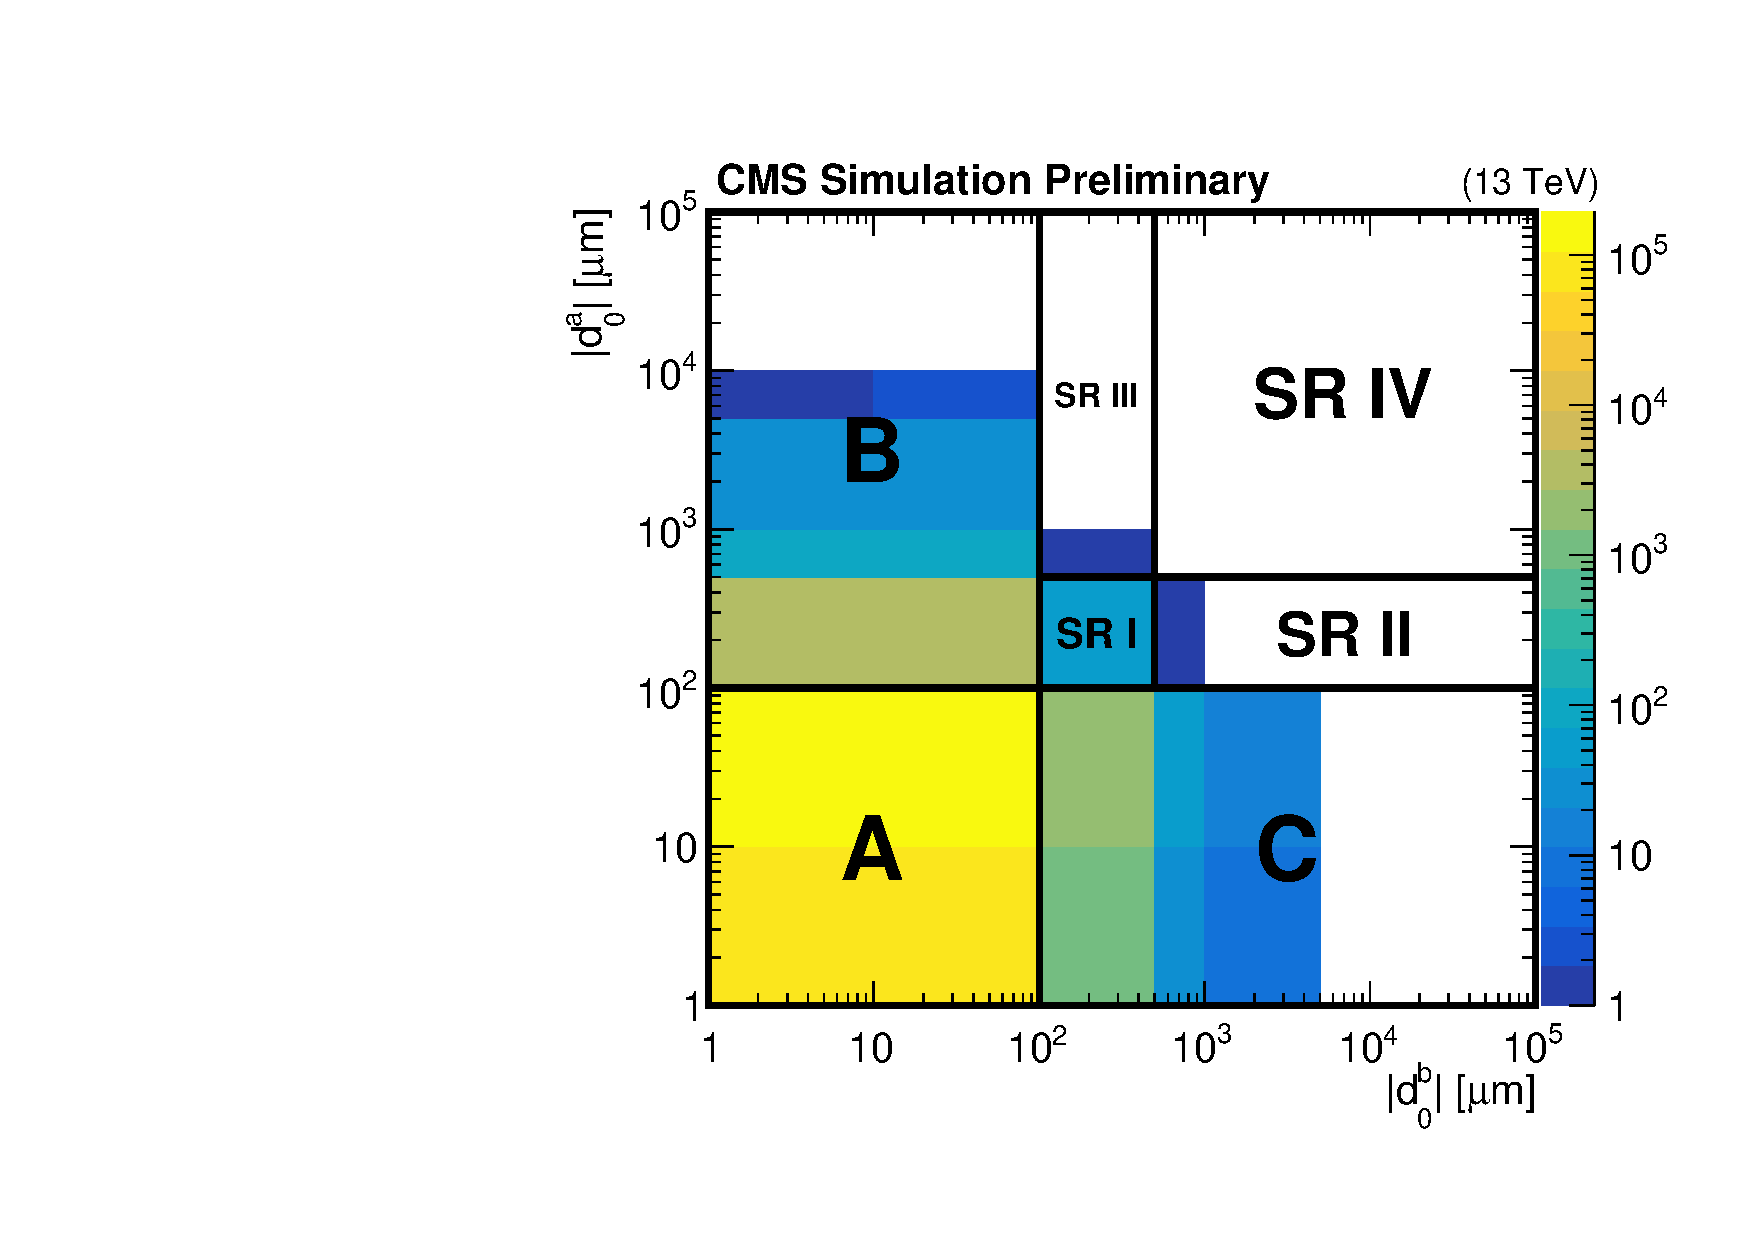
\includegraphics[scale=0.5]{figures/bg/abcdMethod_CMSPreliminary.pdf}
\caption{
A diagram of the ABCD method overlaid on simulated background events passing the 2018 $\Pe\Pgm$ preselection. A, B, and C are control regions, and D is the inclusive SR, which includes SRs I, II, III, and IV. Underflow events are included in the bins along the left and bottom edges. 
}
\label{abcd_regions}
\end{figure}

We then use the number of events in regions A, B, and C to estimate the expected background in each SR. The basic estimation procedure depends on the assumption that \ada and \adb are uncorrelated. If this assumption holds, then $N_{\text{B}}/N_{\text{A}}=N_{\text{D}}/N_{\text{C}}$ and the number of background events in D is equal to $N_{\text{B}}\times N_{\text{C}}/N_{\text{A}}$, where $N_{\text{X}}$ is the number of background events in the given region. We find that \ada and \adb are indeed uncorrelated over much of the \ad-\ad plane, but the correlation discussed in Section~\ref{bg_sources} renders the basic ABCD method insufficient to estimate the background in SR I. After quantifying the degree of correlation in Section~\ref{cr_closure_tests}, we define a procedure to correct the basic ABCD estimate in Section~\ref{abcd_correction}.

In order to maximize sensitivity to a wide range of new particle lifetimes, we further subdivide region D into the following four SRs:
\begin{itemize}
    \itemsep0em
    \item SR I:   $\num{100}\leq\ada<\SI{500}{\um}$, $\num{100} < \adb<\SI{500}{\um}$
    \item SR II:  $\num{100}\leq\ada<\SI{500}{\um}$, $\SI{500}{\um}<\adb<\SI{10}{\cm}$
    \item SR III: $\SI{500}{\um} \leq \ada<\SI{10}{\cm}$, $\num{100} < \adb<\SI{500}{\um}$
    \item SR IV:  $\SI{500}{\um} \leq \ada<\SI{10}{\cm}$, $\SI{500}{\um}<\adb<\SI{10}{\cm}$
\end{itemize}
The exact boundaries between the four SRs are motivated by the expected contributions of the different background sources, as explained in \ref{bg_sources}. This approach also necessitates that the definitions of regions B and C vary in accordance with the SR for which a given estimate is performed (e.g. only the events in the $\num{100}\leq\ada<\SI{500}{\um}$ range of region B are considered when estimating the yields of SR I and II). Finally, we subdivide SR I into two bins using one lepton's \pt to further increase sensitivity to high-mass, low-lifetime new physics. Table~\ref{pt_bins} lists the \pt boundary in each channel and year.

\begin{table}[ht] 
\noindent \centering{}
\topcaption{The \pt boundaries between the low- and high-\pt bins of SR I in each channel.}
\label{pt_bins}
\begin{tabular}{llll}
\hline
  & \pt boundary [\si{\GeV}] \\
\hline
2016 $\Pe\Pgm$       & leading $\Pgm$ $\pt=90$ \\
2017+2018 $\Pe\Pgm$  & leading $\Pgm$ $\pt=140$ \\
2016 $\Pe\Pe$        & leading $\Pe$ $\pt=300$ \\
2017+2018 $\Pe\Pe$   & leading $\Pe$ $\pt=400$ \\
2016 $\Pgm\Pgm$      & leading $\Pgm$ $\pt=100$ \\
2017+2018 $\Pgm\Pgm$ & leading $\Pgm$ $\pt=100$ \\
\hline
\end{tabular}
\end{table}

When performing the background estimate and closure tests, we treat the 2016 data and simulation separately from the 2017--2018 data and simulation to avoid any correlations between \ada and \adb that may arise from the differences between the original and Phase-1 pixel detectors employed by CMS in 2016 and 2017--2018, respectively (see Section~\ref{tracker}).\fxnote{mention largeEtaAndD0 stuff too?}

\subsection{Closure tests in control regions}
\label{cr_closure_tests}
We perform several closure tests of the background estimation procedure in data and simulation to test the method and quantify the degree of \ada-\adb correlation from the processes discussed in \ref{bg_sources}. Two series of tests are performed, the first in the \num{100}--\SI{500}{\um} subregions of regions B and C and the second in the \SI{500}{\um}--\SI{10}{\cm} subregions of regions B and C.

\subsubsection{\num{100}--\SI{500}{\um} tests}
We perform closure tests in subregions of regions B and C where one lepton is more prompt (\num{20}--\SI{100}{\um}) and the other is more displaced (\num{100}--\SI{500}{\um}). In these closure tests, we estimate the background yield using the simple ABCD method and then use the ratio of the actual number of events to the estimated number of events as the measure of nonclosure (and therefore \ada-\adb correlation). With this approach, a ratio of 1 corresponds to closure and no \ada-\adb correlation while ratios greater than 1 correspond to nonclosure and positive \ada-\adb correlation. Using the procedure outlined in Section~\ref{abcd_correction}, we estimate the corresponding degree of nonclosure in SR I by fitting the resulting ratios and extrapolating from the closure test regions to SR I. We perform identical procedures in regions B and C and then average the resulting extrapolated ratios.

Table \ref{100to500um_tests} shows the average extrapolated ratios for three rounds of closure tests: one in background simulation with the \ztautaull events removed, one in the full background simulation, and one in data. The average extrapolated ratios are always compatible with one in background simulation without \ztautaull events, but they generally increase when the \ztautaull events are included. Furthermore, the average extrapolated ratios from the full background simulation generally describe the average extrapolated ratios in data. From these results, we conclude that within our statistical uncertainties, \ztautaull events are the only meaningful source of correlation and that the degree of correlation observed in data is modeled reasonably well in simulation. We also observe that the variation in the degree of correlation across channels matches our expectations: correlation increases with the number of muons in the final state and is greater in 2017--2018 than 2016 because of the improved $d_0$ resolution made possible by the Phase-1 tracker upgrade (described in Section~\ref{tracker}).

\begin{table}
\noindent \centering{}
\topcaption{Closure test results in background simulation (with and without \linebreak[4]\ztautaull events) and in data, in the \num{100}--\SI{500}{\um} region. The average extrapolated ratios and their statistical uncertainties are given. The A, B, C, and D regions are defined as follows: A is 20--\SI{30}{\um} in prompt lepton \ad and 20--\SI{100}{\um} in displaced lepton \ad, B is 20--\SI{30}{\um} in prompt lepton \ad and 100--\SI{500}{\um} in displaced lepton \ad, C is always 20--100\mum in displaced lepton \ad, D (the test region) is always 100--\SI{500}{\um} in displaced lepton \ad, and we perform repeated tests while simultaneously varying the C and D prompt lepton \ad{}s within the 30--\SI{100}{\um} range.}
\label{100to500um_tests}
\begin{tabular}{lccc}
\hline
&\multirow{2}{*}{\begin{tabular}[c]{@{}c@{}}Bkg. simulation\\without \ztautaull\end{tabular}} &\multirow{2}{*}{\begin{tabular}[c]{@{}c@{}}Full bkg.      \\simulation\end{tabular}} & \multirow{2}{*}{Data}\\
& & & \\
  \hline
2016 $\Pe\Pgm$       & $0.9\pm0.3$ & $1.6\pm0.6$ & $0.9\pm1.3$\\
2017+2018 $\Pe\Pgm$  & $1.1\pm0.4$ & $1.6\pm0.7$ & $3.1\pm1.0$\\
2016 $\Pe\Pe$        & $0.8\pm0.5$ & $0.8\pm0.5$ & $0.6\pm0.6$\\
2017+2018 $\Pe\Pe$   & $0.8\pm1.0$ & $1.6\pm0.9$ & $1.5\pm0.4$\\
2016 $\Pgm\Pgm$      & $1.1\pm0.8$ & $2.0\pm0.8$ & $2.5\pm1.0$\\
2017+2018 $\Pgm\Pgm$ & $2.6\pm2.8$ & $7.8\pm3.7$ & $4.2\pm1.8$\\
\hline
Average              & $1.2\pm0.5$ & $2.6\pm0.7$ & $2.1\pm0.5$\\ 
\hline
\end{tabular}
\end{table}

\subsubsection{\SI{500}{\um}--\SI{10}{\cm} tests}
We next perform closure tests in subregions of regions B and C where one lepton is more prompt (\num{20}--\SI{100}{\um}) and the other is more displaced (\SI{500}{\um}--\SI{10}{\cm}). We again use the ratio of the actual number of events to the estimated number of events as the measure of nonclosure, but in these tests we expect the ratio to be consistent with one because \ztautaull events do not contribute meaningfully beyond \SI{500}{\um}. Table \ref{500umto10cm_tests} shows that this is indeed the case for background simulation (with and without \ztautaull events) and for data. These results imply that \ada and \adb are uncorrelated beyond \SI{500}{\um}, which means that a simple ABCD procedure will be adequate for estimating the background yields in SRs II, III, and IV.

\begin{table}[ht] 
\renewcommand{\arraystretch}{1.3}
\noindent \centering{}
\topcaption{Closure test results in in data and background simulation (with and without \ztautaull events), in the 500\mum--10\cm region. The ratios of the actual yield to the estimated yield and their statistical uncertainties are given. The A, B, C, and D regions are defined as follows: A is 20--30\mum in prompt lepton \ad and 20--100\mum in displaced lepton \ad, B is 20--30\mum in prompt lepton \ad and 500\mum--10\cm in displaced lepton \ad, C is 30--100\mum in prompt lepton \ad and 20--100\mum in displaced lepton \ad, and D (the test region) is 30--100\mum in prompt lepton \ad and 500\mum--10\cm in displaced lepton \ad.}
\label{500umto10cm_tests}
\begin{tabular}{llll}
\hline
  \multicolumn{4}{c}{Region B}\\
  & {\begin{tabular}[l]{@{}l@{}}Bkg. simulation\\w/o \ztautaull\end{tabular}}
  & {\begin{tabular}[l]{@{}l@{}}Bkg.\\simulation\end{tabular}} 
  & Data\\
\hline
2016 $\Pe\Pgm$       & $1.1\pm0.3$         & $1.1\pm0.3$         & $0.4^{+1.0}_{-0.4}$\\
2017+2018 $\Pe\Pgm$  & $0.9^{+0.3}_{-0.2}$ & $0.9^{+0.3}_{-0.2}$ & $0.7\pm0.3$        \\
2016 $\Pe\Pe$        & $0.4^{+0.6}_{-0.3}$ & $0.4^{+0.6}_{-0.3}$ & $1.4^{+1.6}_{-0.9}$\\
2017+2018 $\Pe\Pe$   & $0.5^{+0.8}_{-0.4}$ & $0.3^{+0.4}_{-0.2}$ & $1.0\pm0.3$        \\
2016 $\Pgm\Pgm$      & $0.7\pm0.3$         & $0.7\pm0.3$         & $0.8\pm0.3$        \\
2017+2018 $\Pgm\Pgm$ & $0.8^{+1.8}_{-0.7}$ & $0.4^{+1.0}_{-0.4}$ & $1.8^{+0.6}_{-0.7}$\\
\hline
  \multicolumn{4}{c}{Region C}\\
  & {\begin{tabular}[l]{@{}l@{}}Bkg. simulation\\w/o \ztautaull\end{tabular}}
  & {\begin{tabular}[l]{@{}l@{}}Bkg.\\simulation\end{tabular}} 
  & Data\\
\hline
2016 $\Pe\Pgm$       & $0.8^{+0.4}_{-0.3}$ & $0.8^{+0.4}_{-0.3}$ & $1.0$ (0 vs 0)      \\
2017+2018 $\Pe\Pgm$  & $0.8^{+0.3}_{-0.2}$ & $0.8^{+0.3}_{-0.2}$ & $0.7^{+1.3}_{-0.7}$ \\
2016 $\Pe\Pe$        & $4.0^{+5.8}_{-3.1}$ & $4.0^{+5.8}_{-3.1}$ & $0.7^{+1.0}_{-0.6}$ \\
2017+2018 $\Pe\Pe$   & $3.5^{+2.6}_{-1.8}$ & $2.1^{+2.6}_{-1.5}$ & $1.0\pm0.3$         \\
2016 $\Pgm\Pgm$      & $1.2^{+0.5}_{-0.4}$ & $1.3^{+0.6}_{-0.4}$ & $0.6^{+0.4}_{-0.3}$ \\
2017+2018 $\Pgm\Pgm$ & $0.4^{+0.4}_{-0.3}$ & $0.5^{+0.5}_{-0.3}$ & $0.5^{+0.3}_{-0.2}$ \\
\hline
\end{tabular}
\end{table}


\subsection{ABCD correction and systematic uncertainty}
\label{abcd_correction}
The closure tests of Section~\ref{cr_closure_tests} show that \ada and \adb are frequently positively correlated in the \num{100}--\SI{500}{\um} region but are uncorrelated otherwise. To account for this correlation as well as other possible unforeseen sources of nonclosure, we define a procedure to correct the simple ABCD estimate in SR I and assign a systematic uncertainty to the simple ABCD estimate in all SRs.

\subsubsection{\num{100}--\SI{500}{\um} correction and systematic uncertainty}
\fxnote{would be nice to explain a little more up front}
Figures~\ref{100to500um_fits_emu}, \ref{100to500um_fits_ee}, and \ref{100to500um_fits_mumu} show the results of the data closure tests in the \Pe\Pgm\, \Pe\Pe, and \Pgm\Pgm\ channels, respectively, in the one-prompt (\num{20}--\SI{100}{\um})/one-displaced (\num{100}-\SI{500}{\um}) sidebands. These plots show the ratio of the actual to the estimated number of events as a function of the prompt lepton \ad. In all of these plots, the binning of the prompt lepton axis is initially \SI{10}{\um} wide. Starting from most-displaced bin, we test to see if any bin has fewer than 5 events, and if so, we combine it with whichever neighboring bin has fewer events, repeating until all bins have at least 5 events.

In each of the two sidebands, we then fit the resulting ratios with a straight line, where the slope and y-intercept are allowed to vary, and extrapolate the fit to \SI{200}{\um}, which is where we expect the largest contribution from tau lepton decays (see Section~\ref{bg_sources}). \SI{200}{\um} also happens to be approximately the center-of-mass of the \num{100}--\SI{500}{\um} bin in background simulation. We average the two extrapolated ratios and derive a correction and systematic uncertainty from this average extrapolated ratio.


\begin{figure}[hbtp]
\centering
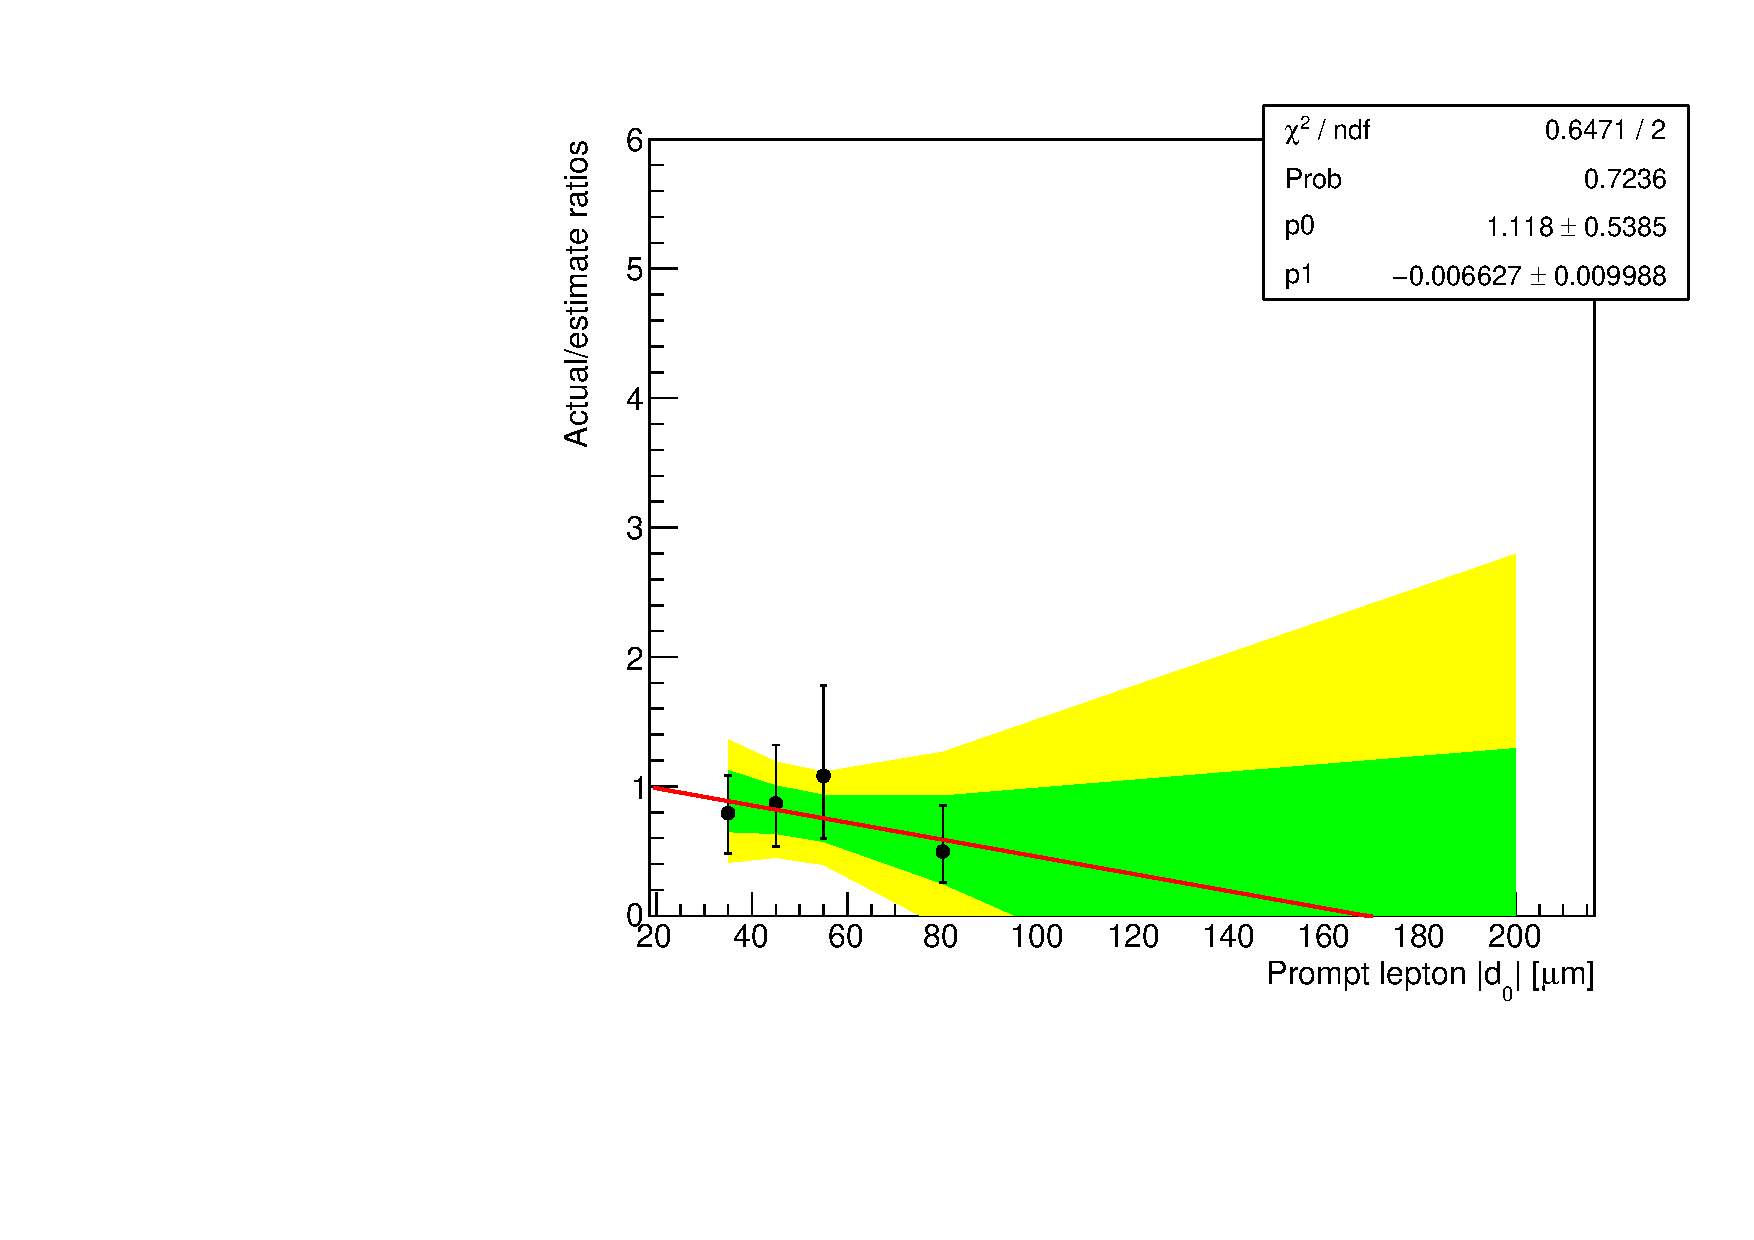
\includegraphics[scale=0.35]{figures/bg/emu_data_2016_displacedMuon_ratiosVsPromptD0.pdf}
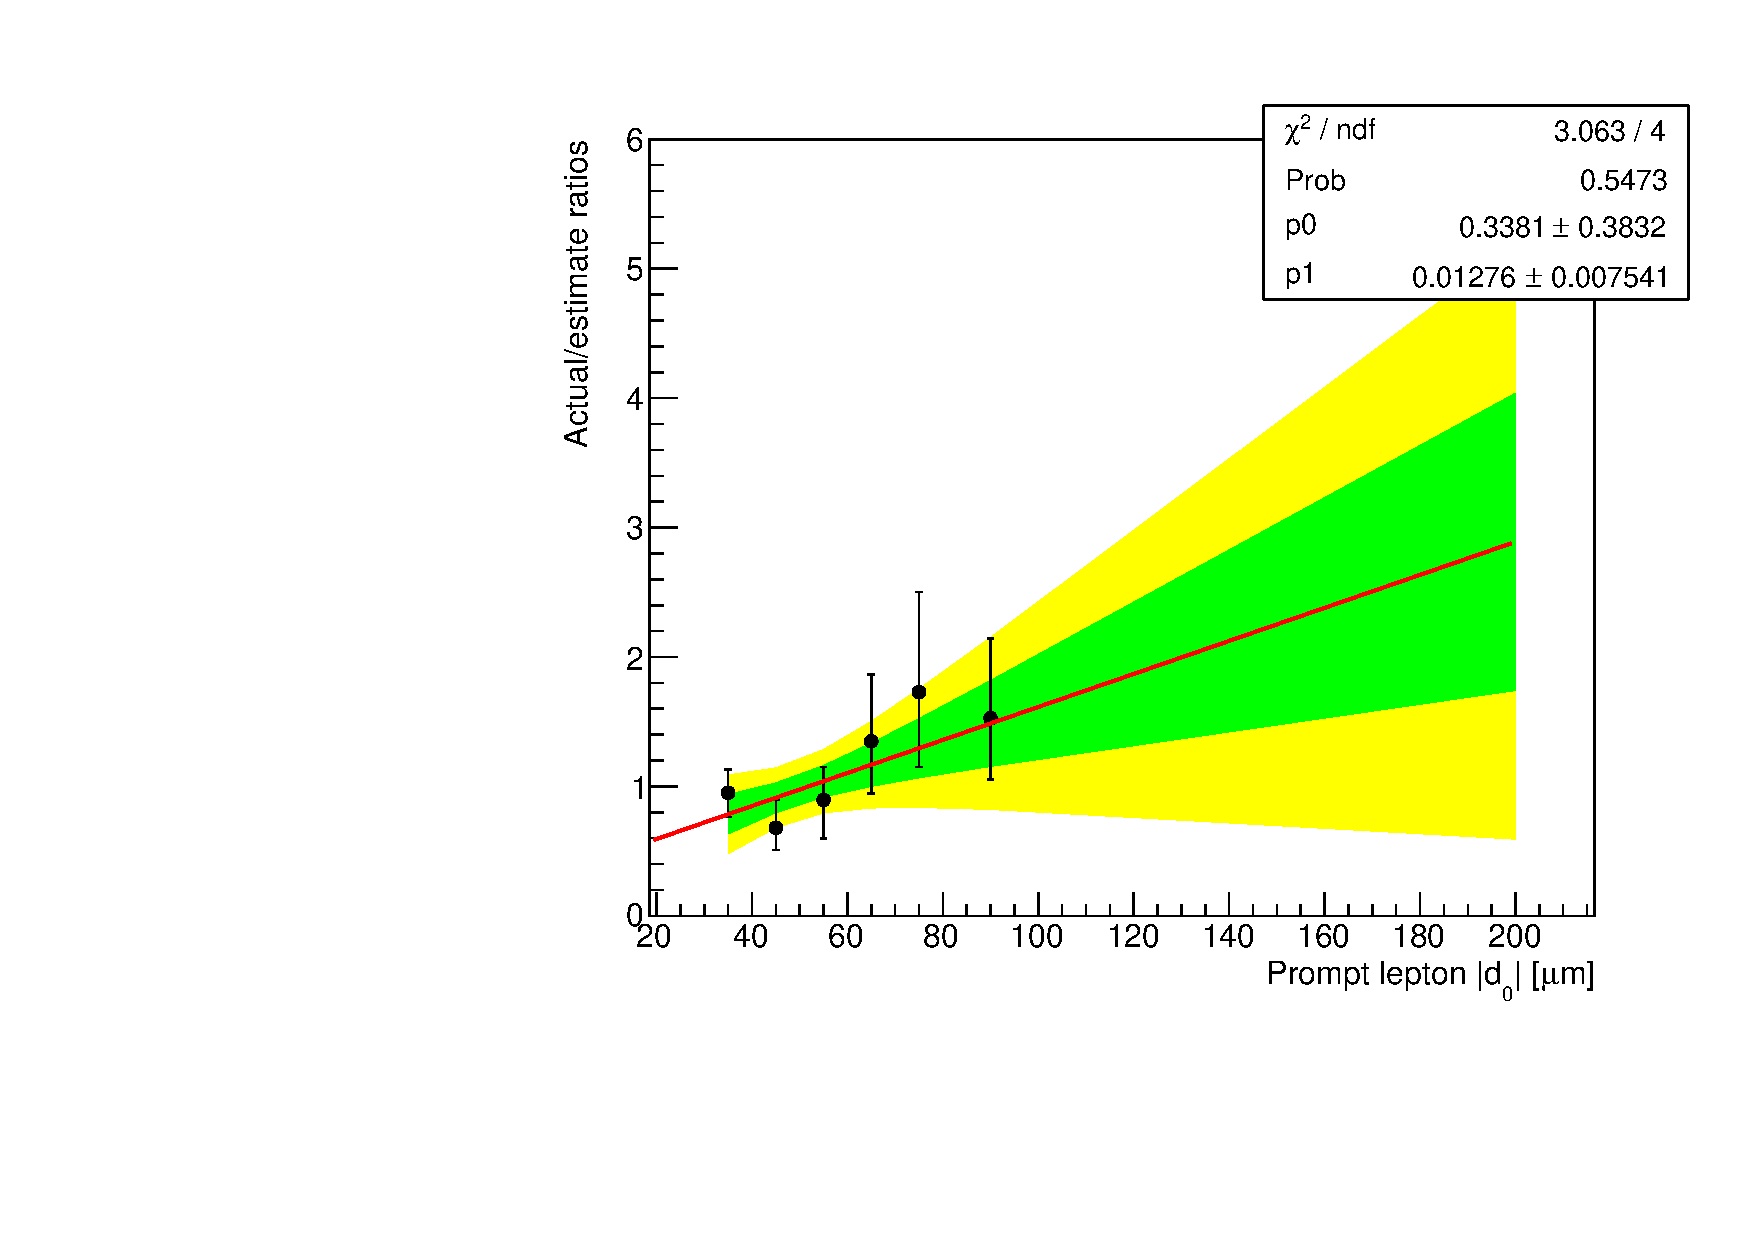
\includegraphics[scale=0.35]{figures/bg/emu_data_2017_2018_displacedMuon_ratiosVsPromptD0.pdf}
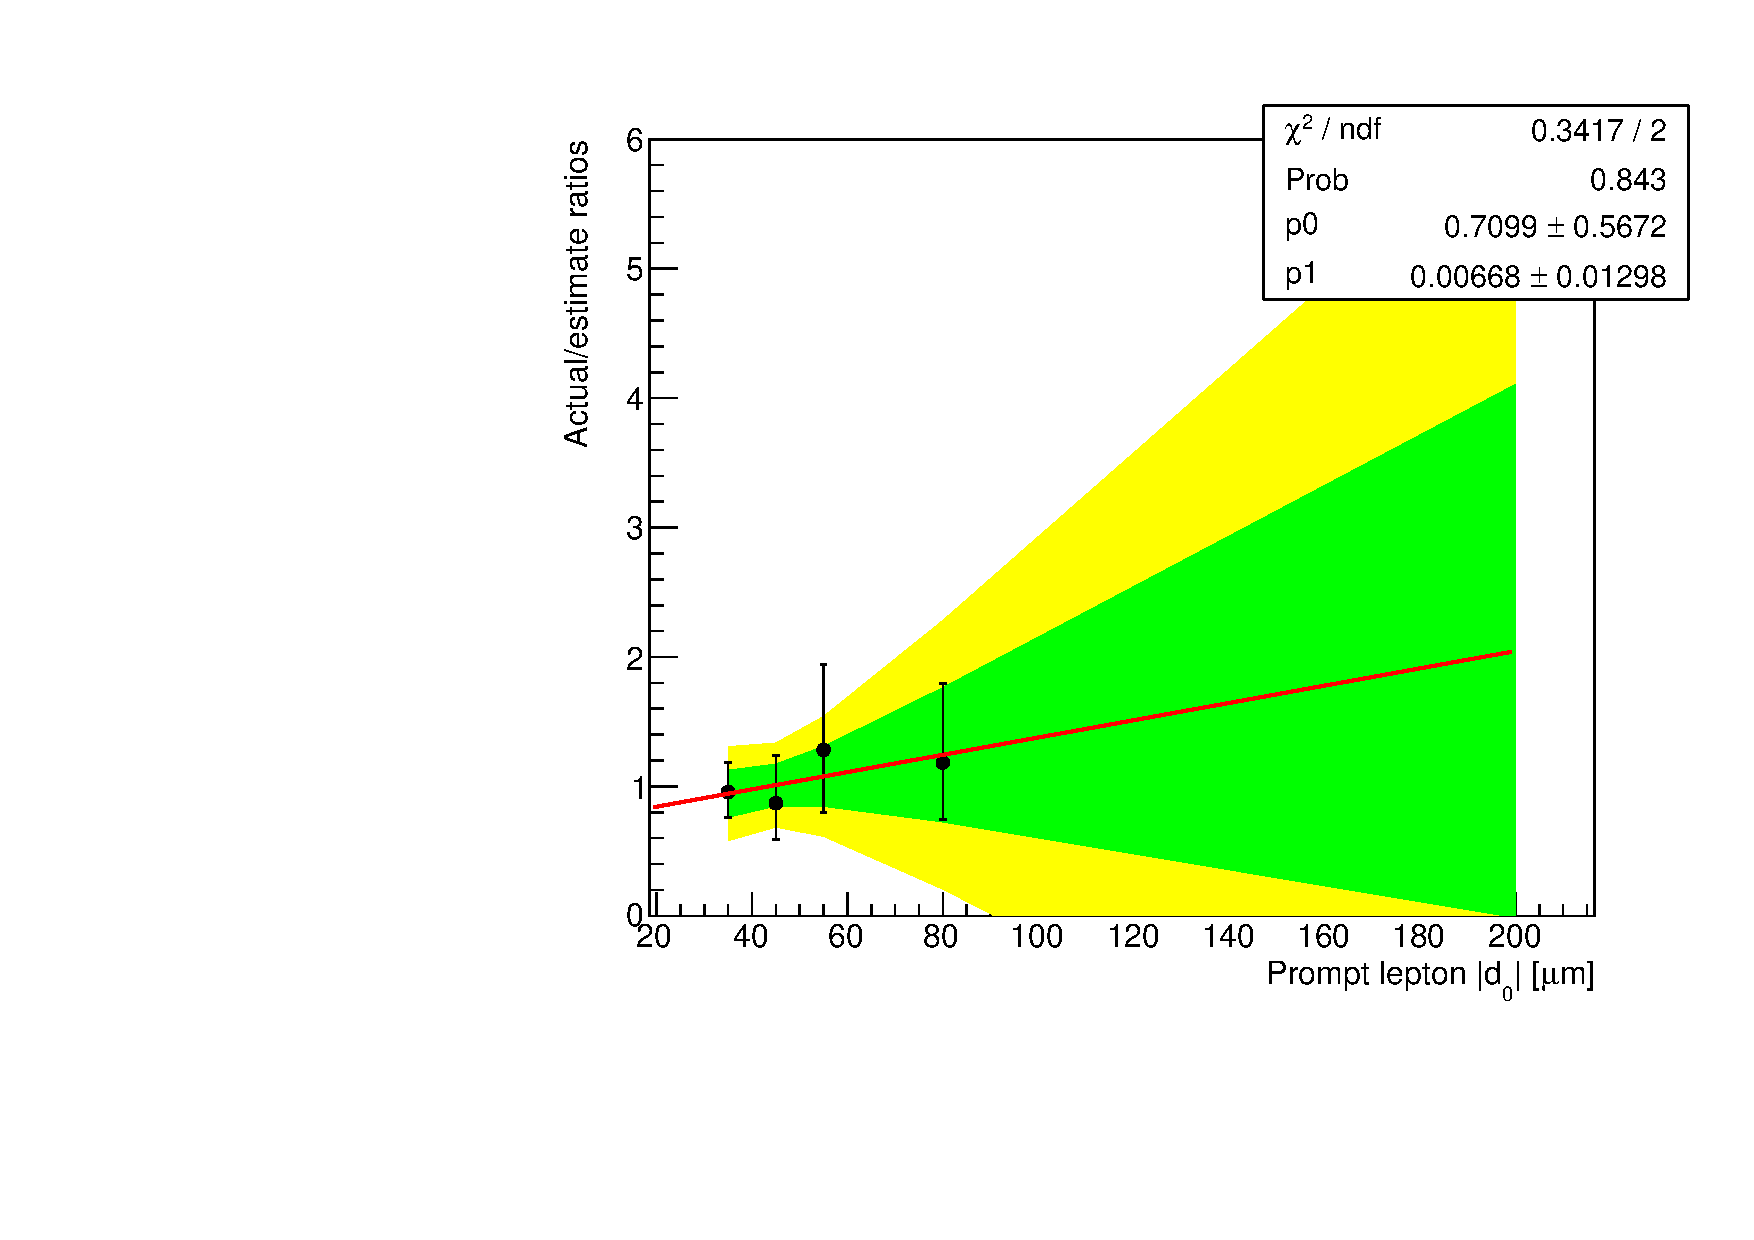
\includegraphics[scale=0.35]{figures/bg/emu_data_2016_displacedElectron_ratiosVsPromptD0.pdf}
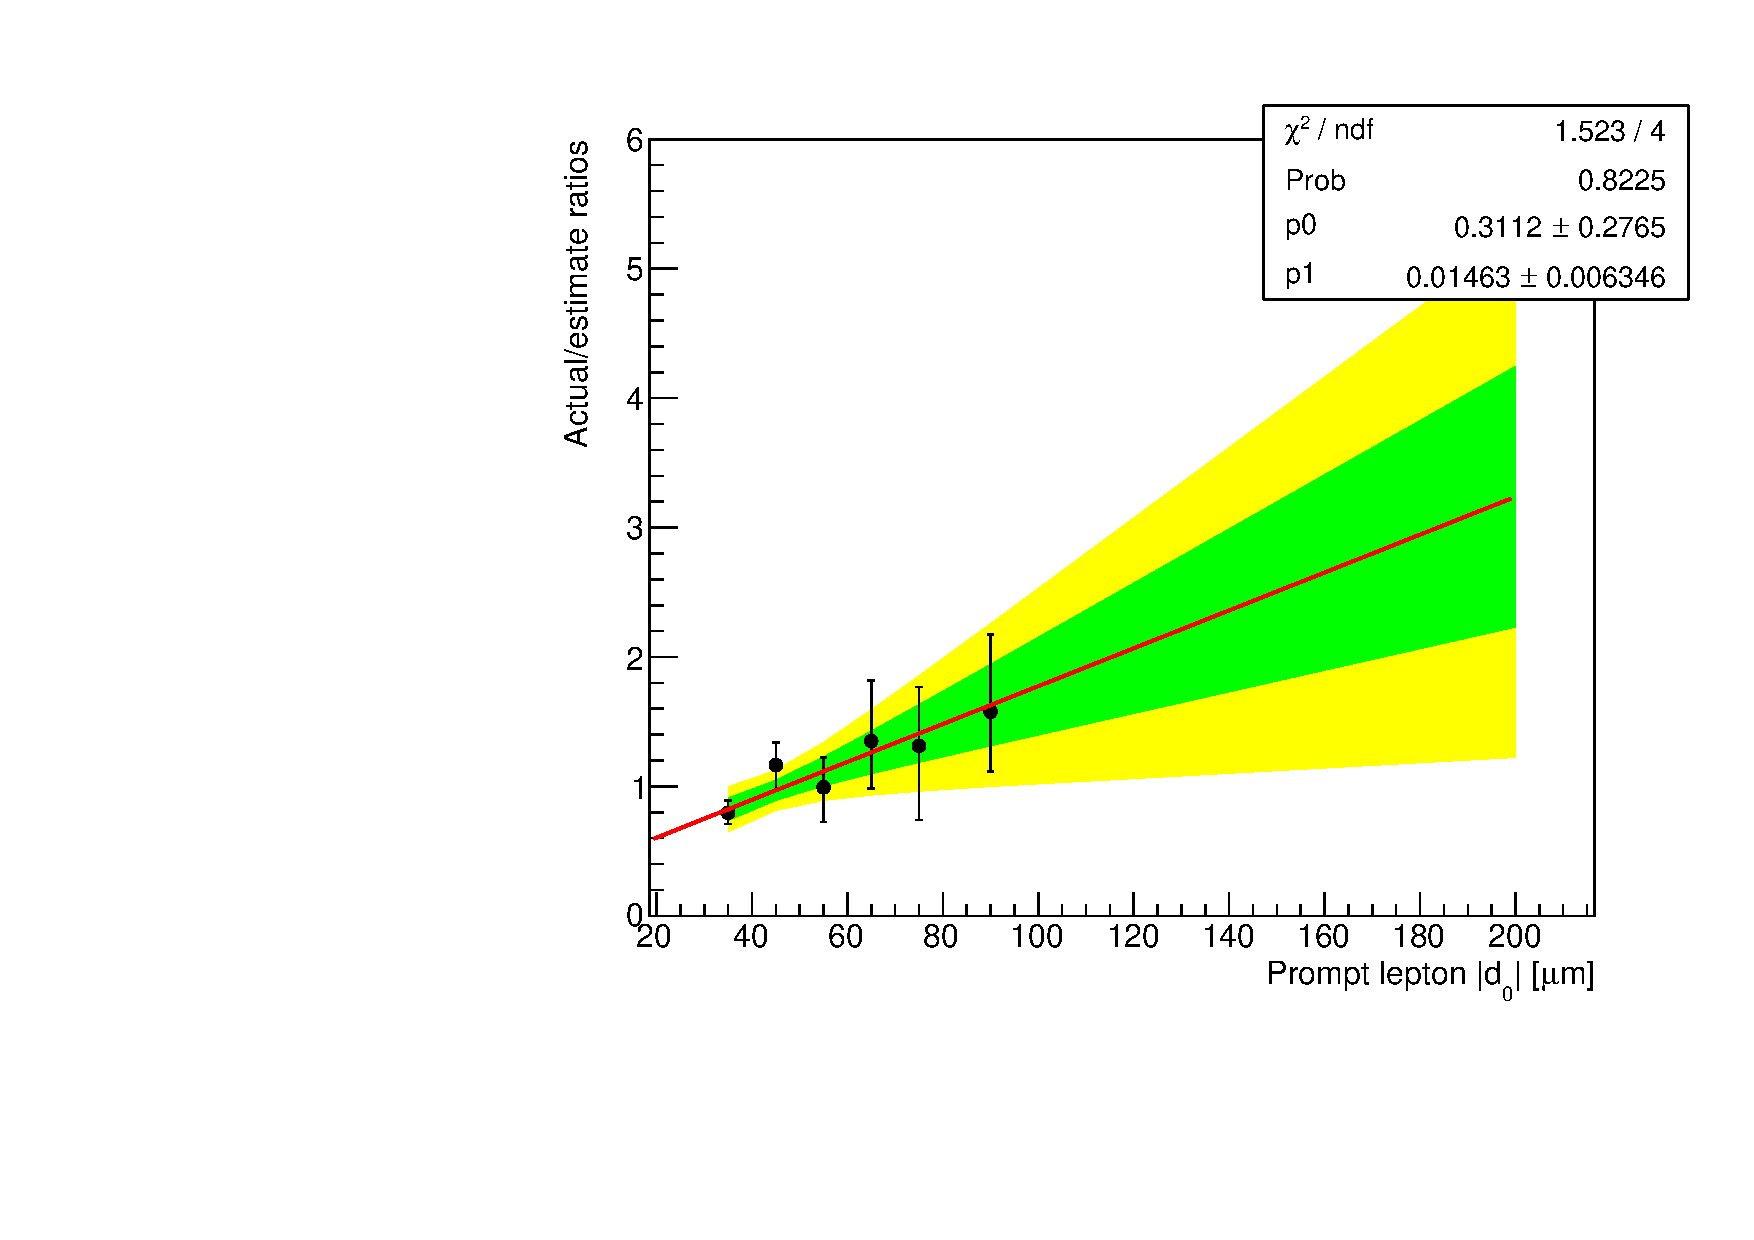
\includegraphics[scale=0.35]{figures/bg/emu_data_2017_2018_displacedElectron_ratiosVsPromptD0.pdf}
\caption{Background estimation closure tests in data, in the one-prompt (20--100\mum)/one-displaced (100-500\mum) sidebands, in the $\Pe\Pgm$ channel. The prompt-leading-electron/displaced-leading-muon sideband is shown in the upper row, and the prompt-leading-muon/displaced-leading-electron sideband is shown in the lower row. The plots on the left show the results for 2016 data, and the plots on the right are for combined 2017 and 2018 data. The plots show the ratio of the actual to the estimated number of events as a function of the prompt lepton \ad. The data are fitted with a straight line, where the slope and y-intercept are allowed to vary. The $1\sigma$ and $2\sigma$ confidence intervals are shown in the green and yellow bands, respectively.}\fxnote{update to d0a, d0b or B, C language}
\label{100to500um_fits_emu}
\end{figure}


\begin{figure}[hbtp]
\centering
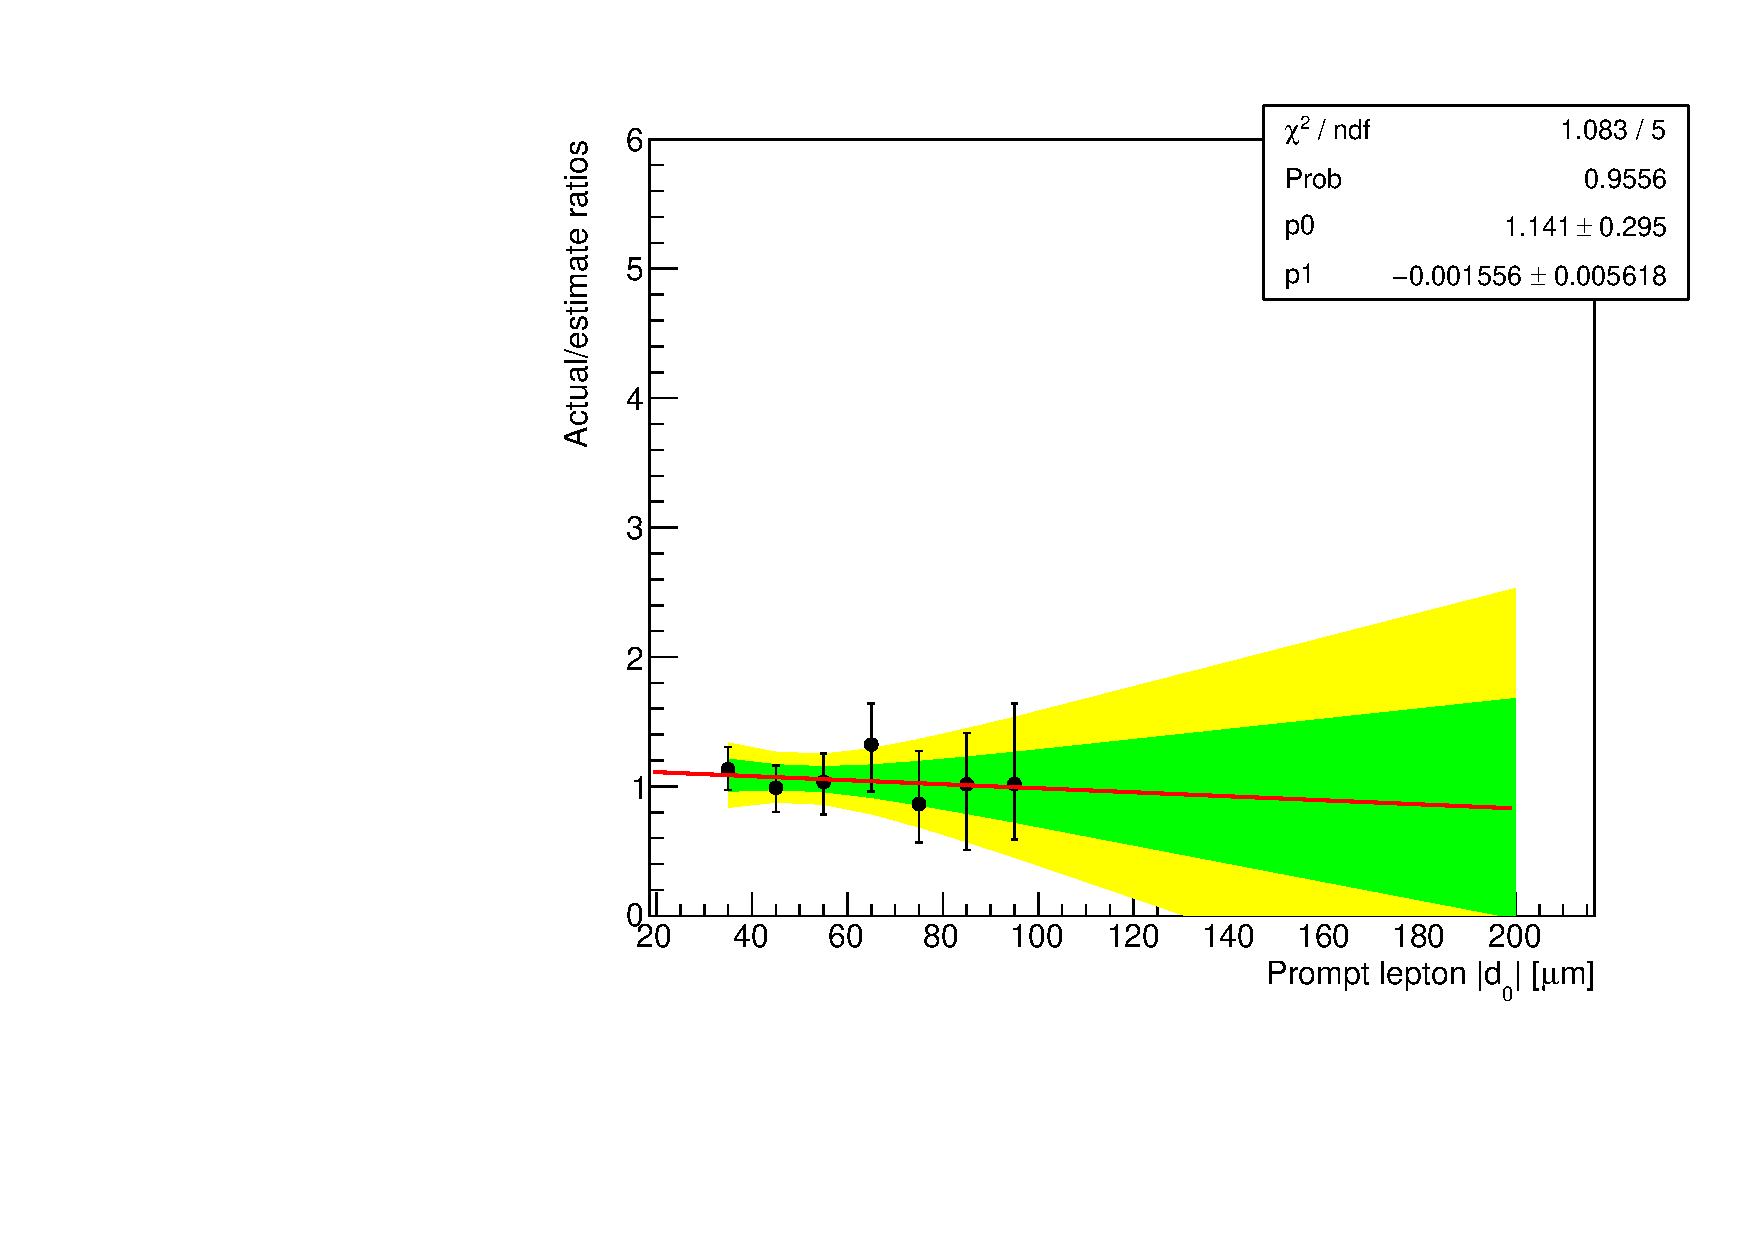
\includegraphics[scale=0.35]{figures/bg/ee_data_2016_displacedSubleading_ratiosVsPromptD0.pdf}
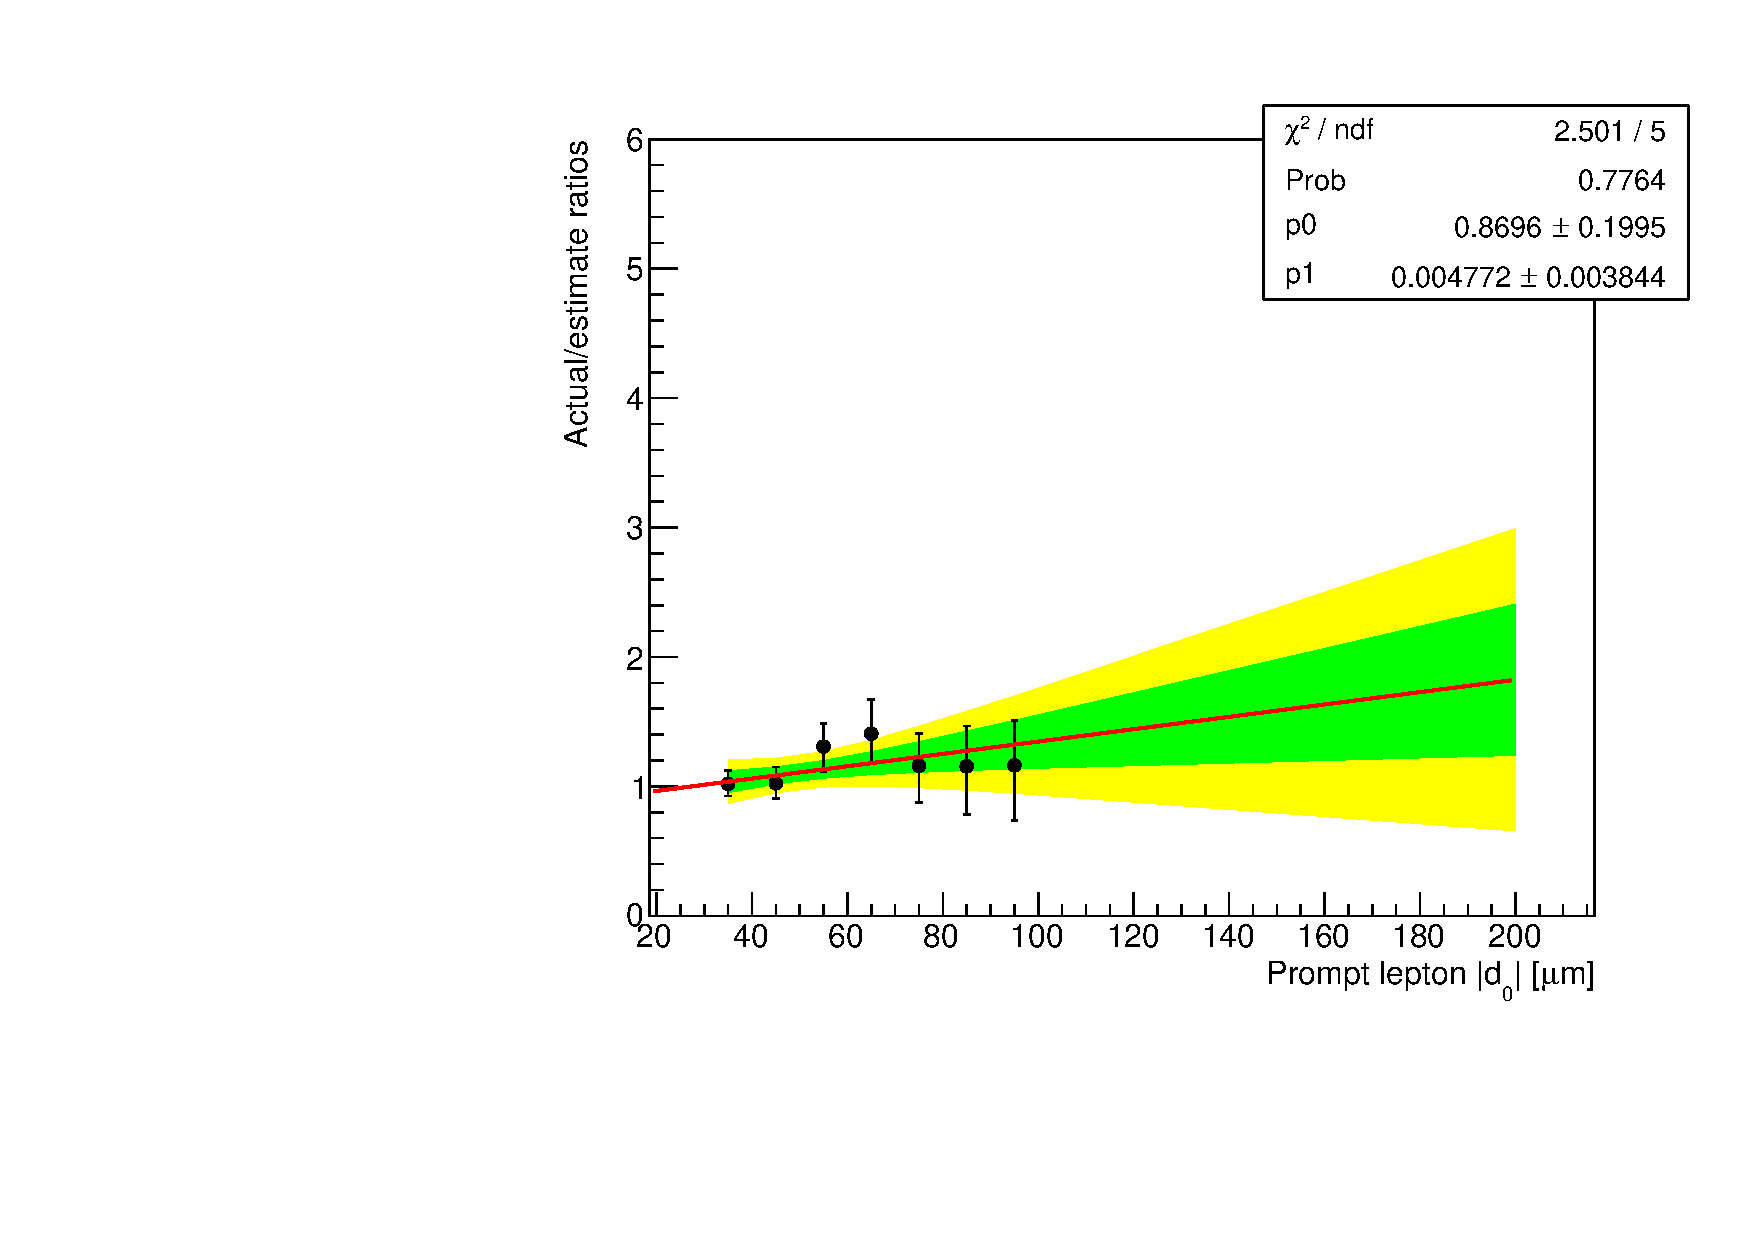
\includegraphics[scale=0.35]{figures/bg/ee_data_2017_2018_displacedSubleading_ratiosVsPromptD0.pdf}
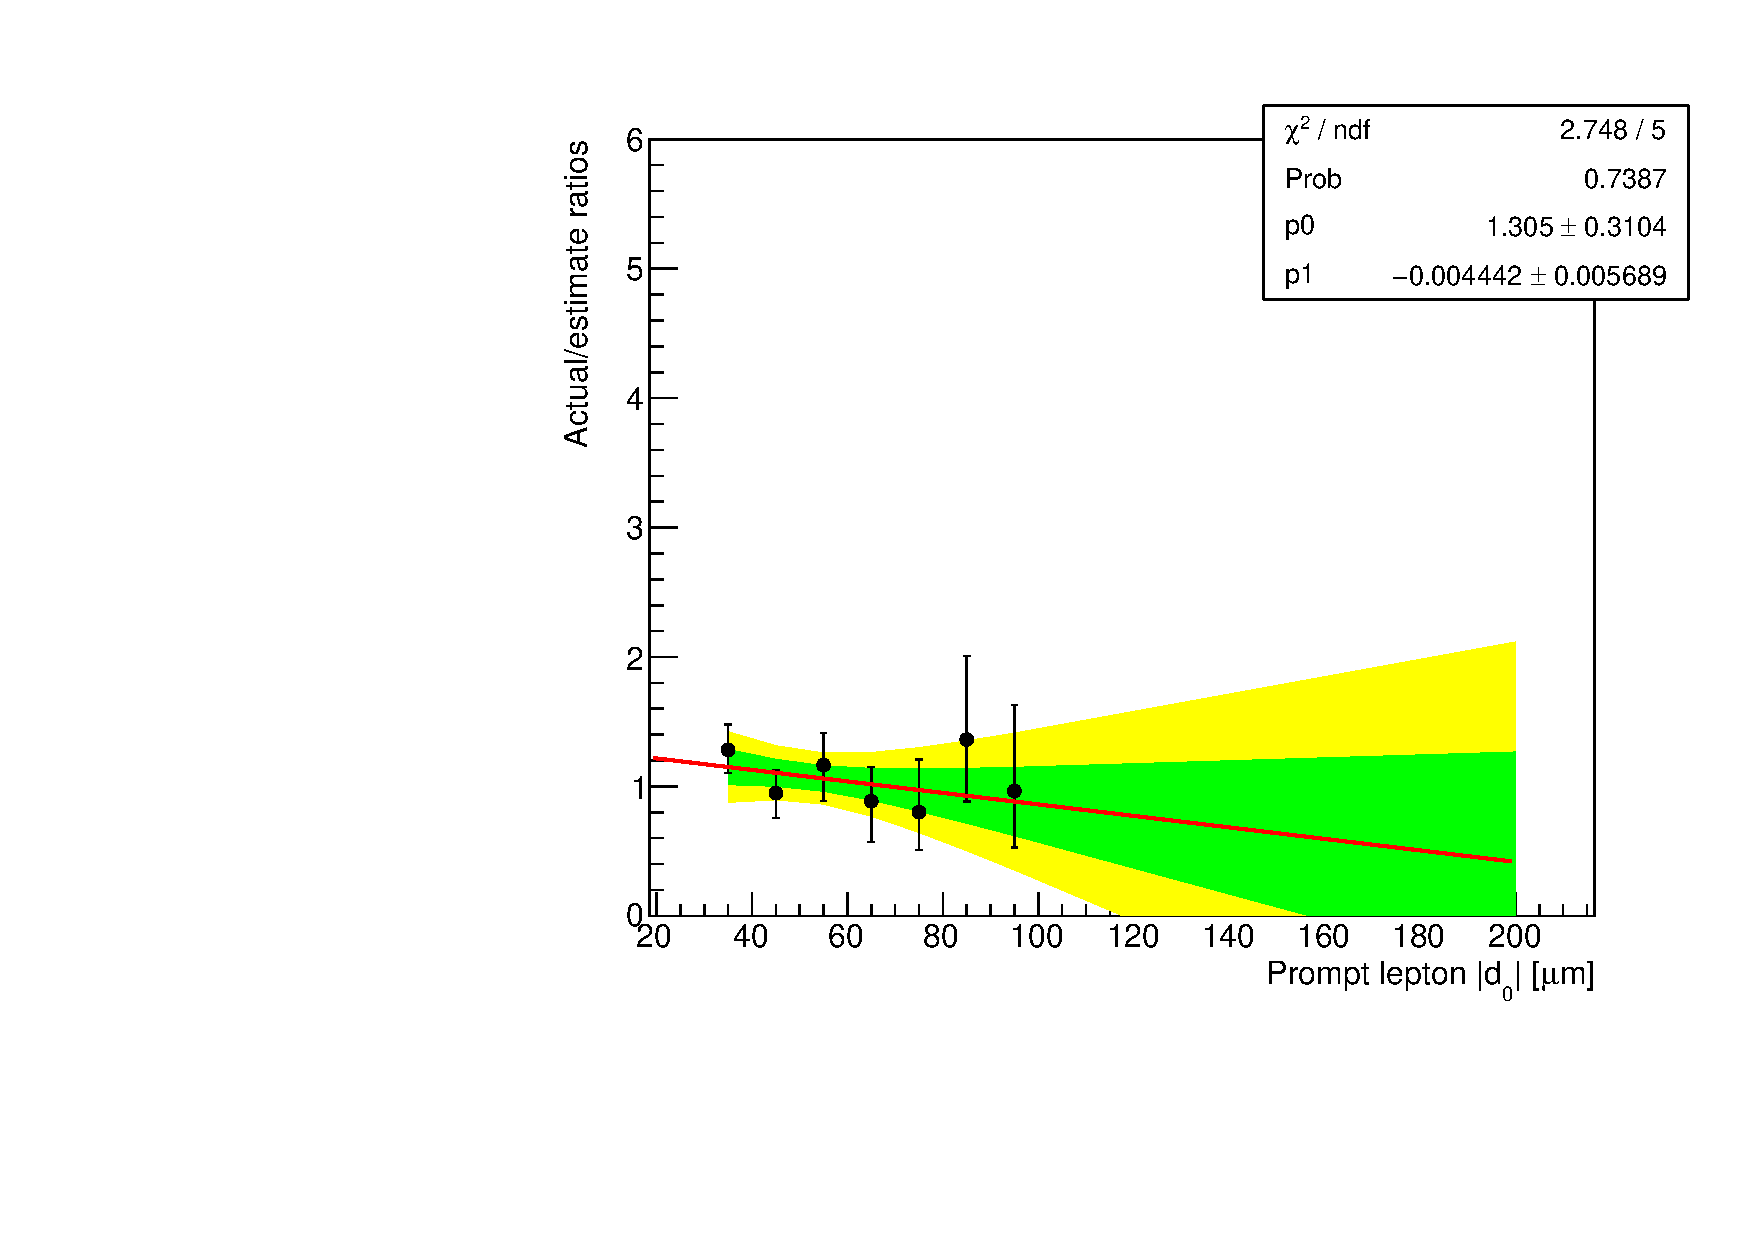
\includegraphics[scale=0.35]{figures/bg/ee_data_2016_displacedLeading_ratiosVsPromptD0.pdf}
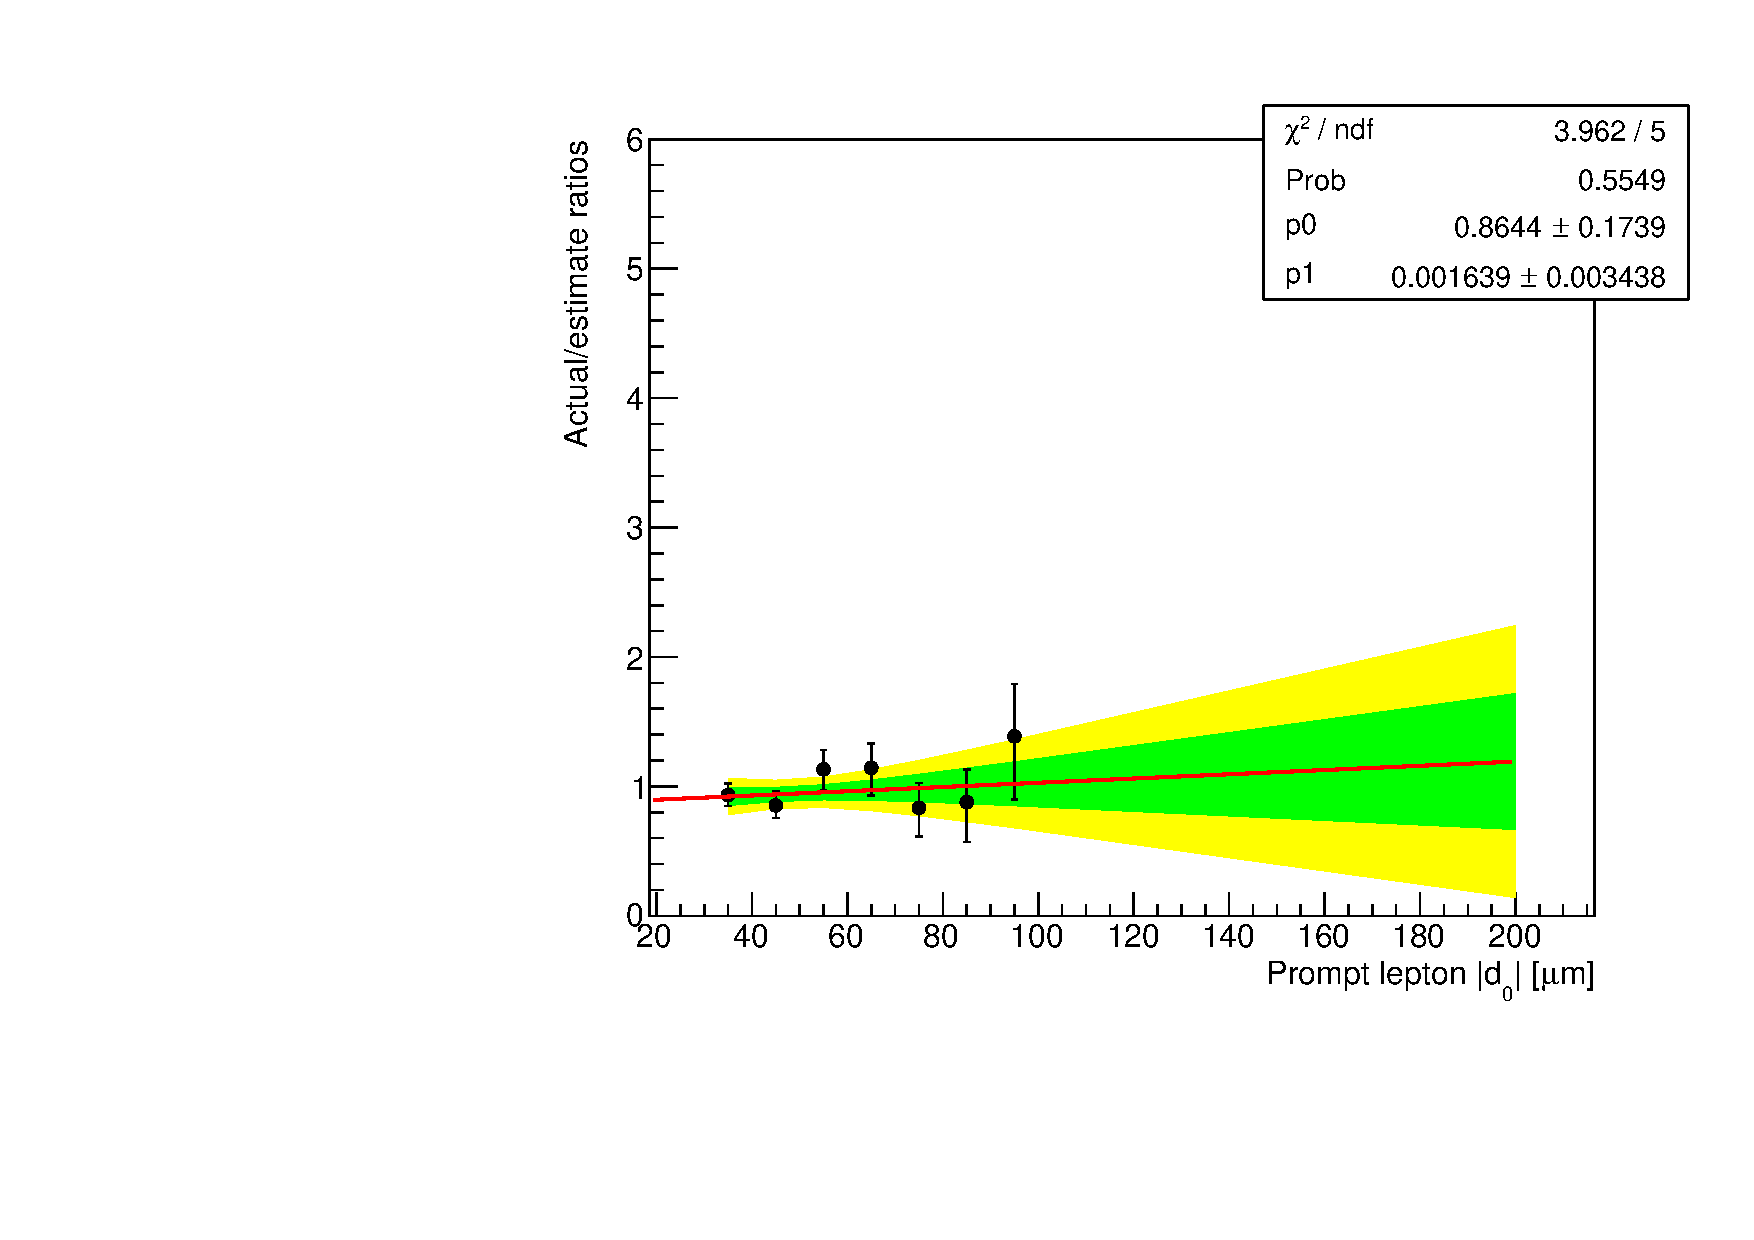
\includegraphics[scale=0.35]{figures/bg/ee_data_2017_2018_displacedLeading_ratiosVsPromptD0.pdf}
\caption{Background estimation closure tests in data, in the one-prompt (20--100\mum)/one-displaced (100-500\mum) sidebands, in the $\Pe\Pe$ channel. The prompt-leading-electron/displaced-subleading-electron sideband is shown in the upper row, and the prompt-subleading-electron/displaced-leading-electron sideband is shown in the lower row. The plots on the left show the results for 2016 data, and the plots on the right are for combined 2017 and 2018 data. The plots show the ratio of the actual to the estimated number of events as a function of the prompt lepton \ad. The data are fitted with a straight line, where the slope and y-intercept are allowed to vary. The $1\sigma$ and $2\sigma$ confidence intervals are shown in the green and yellow bands, respectively.}\fxnote{update to d0a, d0b or B, C language}
\label{100to500um_fits_ee}
\end{figure}


\begin{figure}[hbtp]
\centering
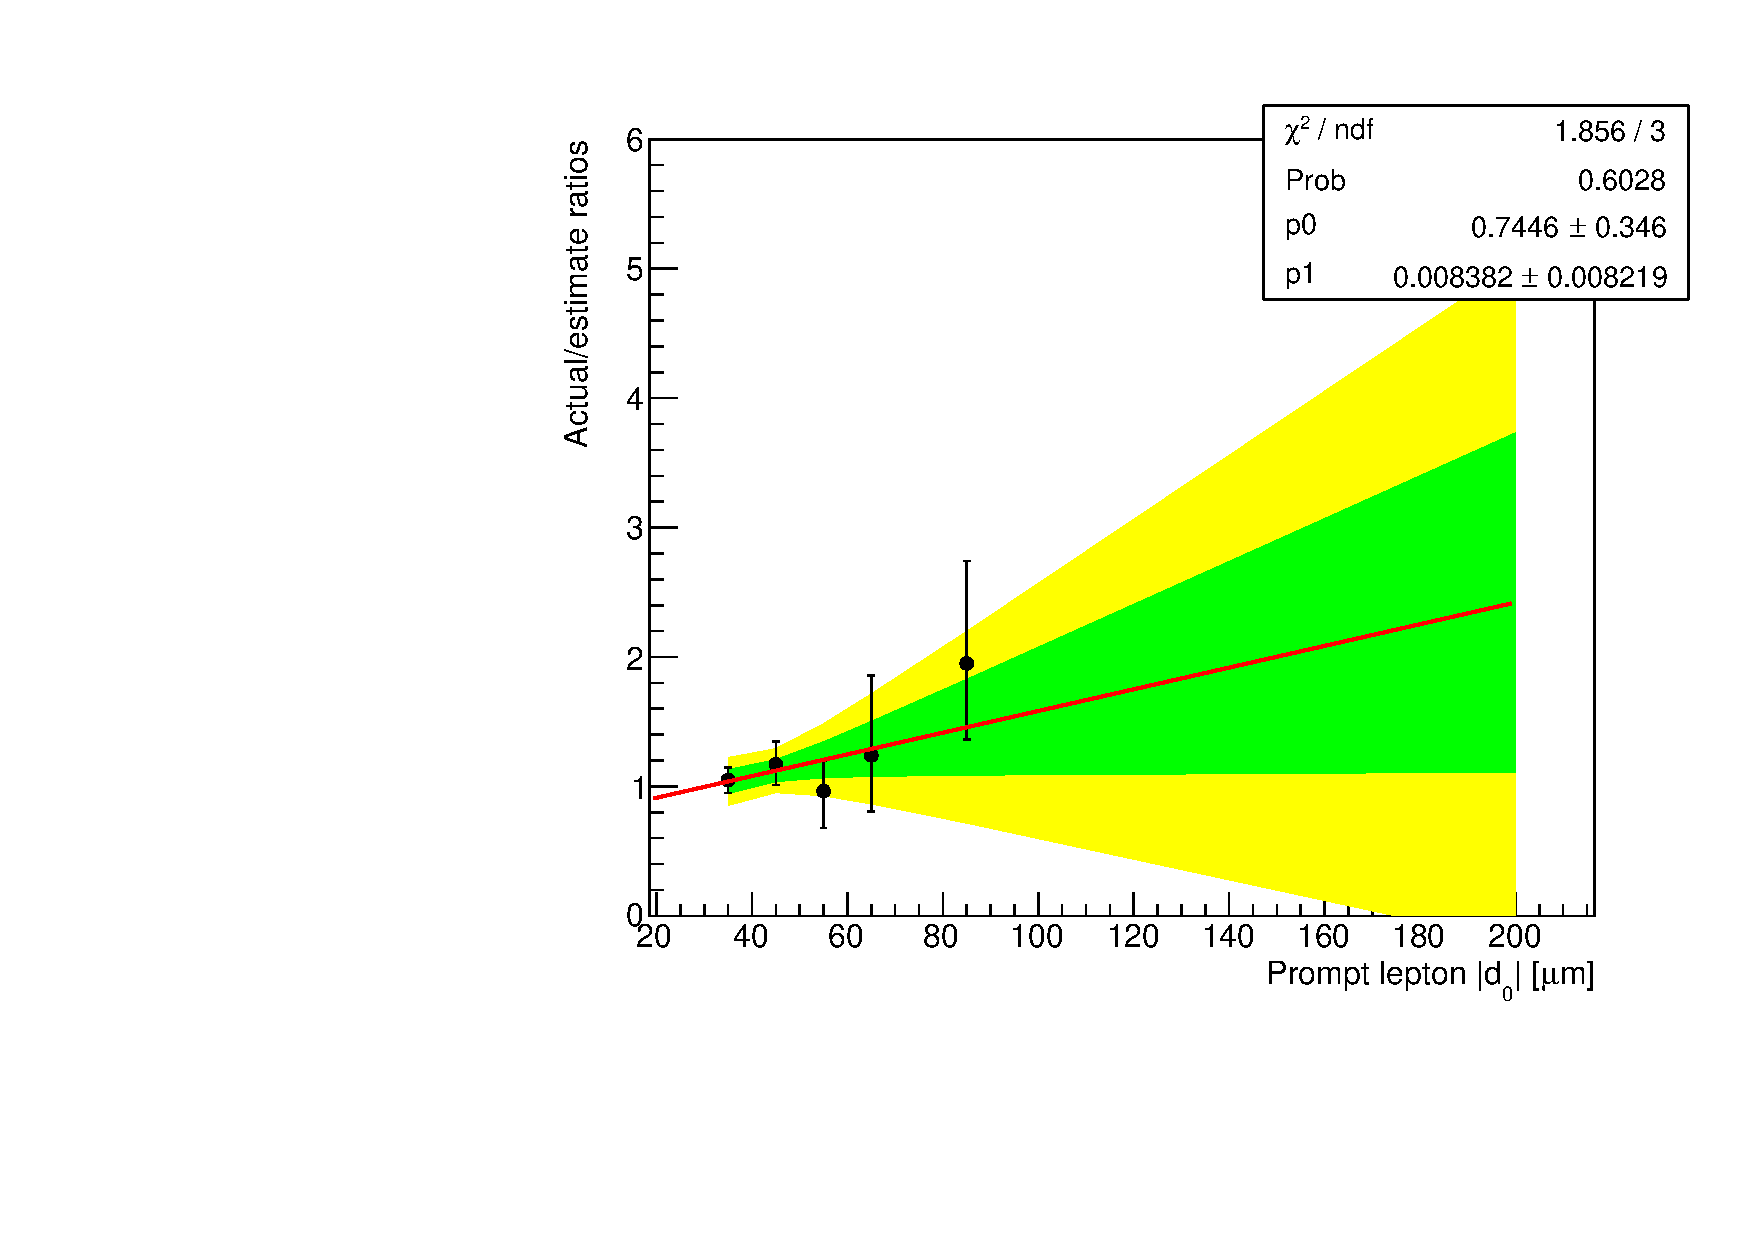
\includegraphics[scale=0.35]{figures/bg/mumu_data_2016_displacedSubleading_ratiosVsPromptD0.pdf}
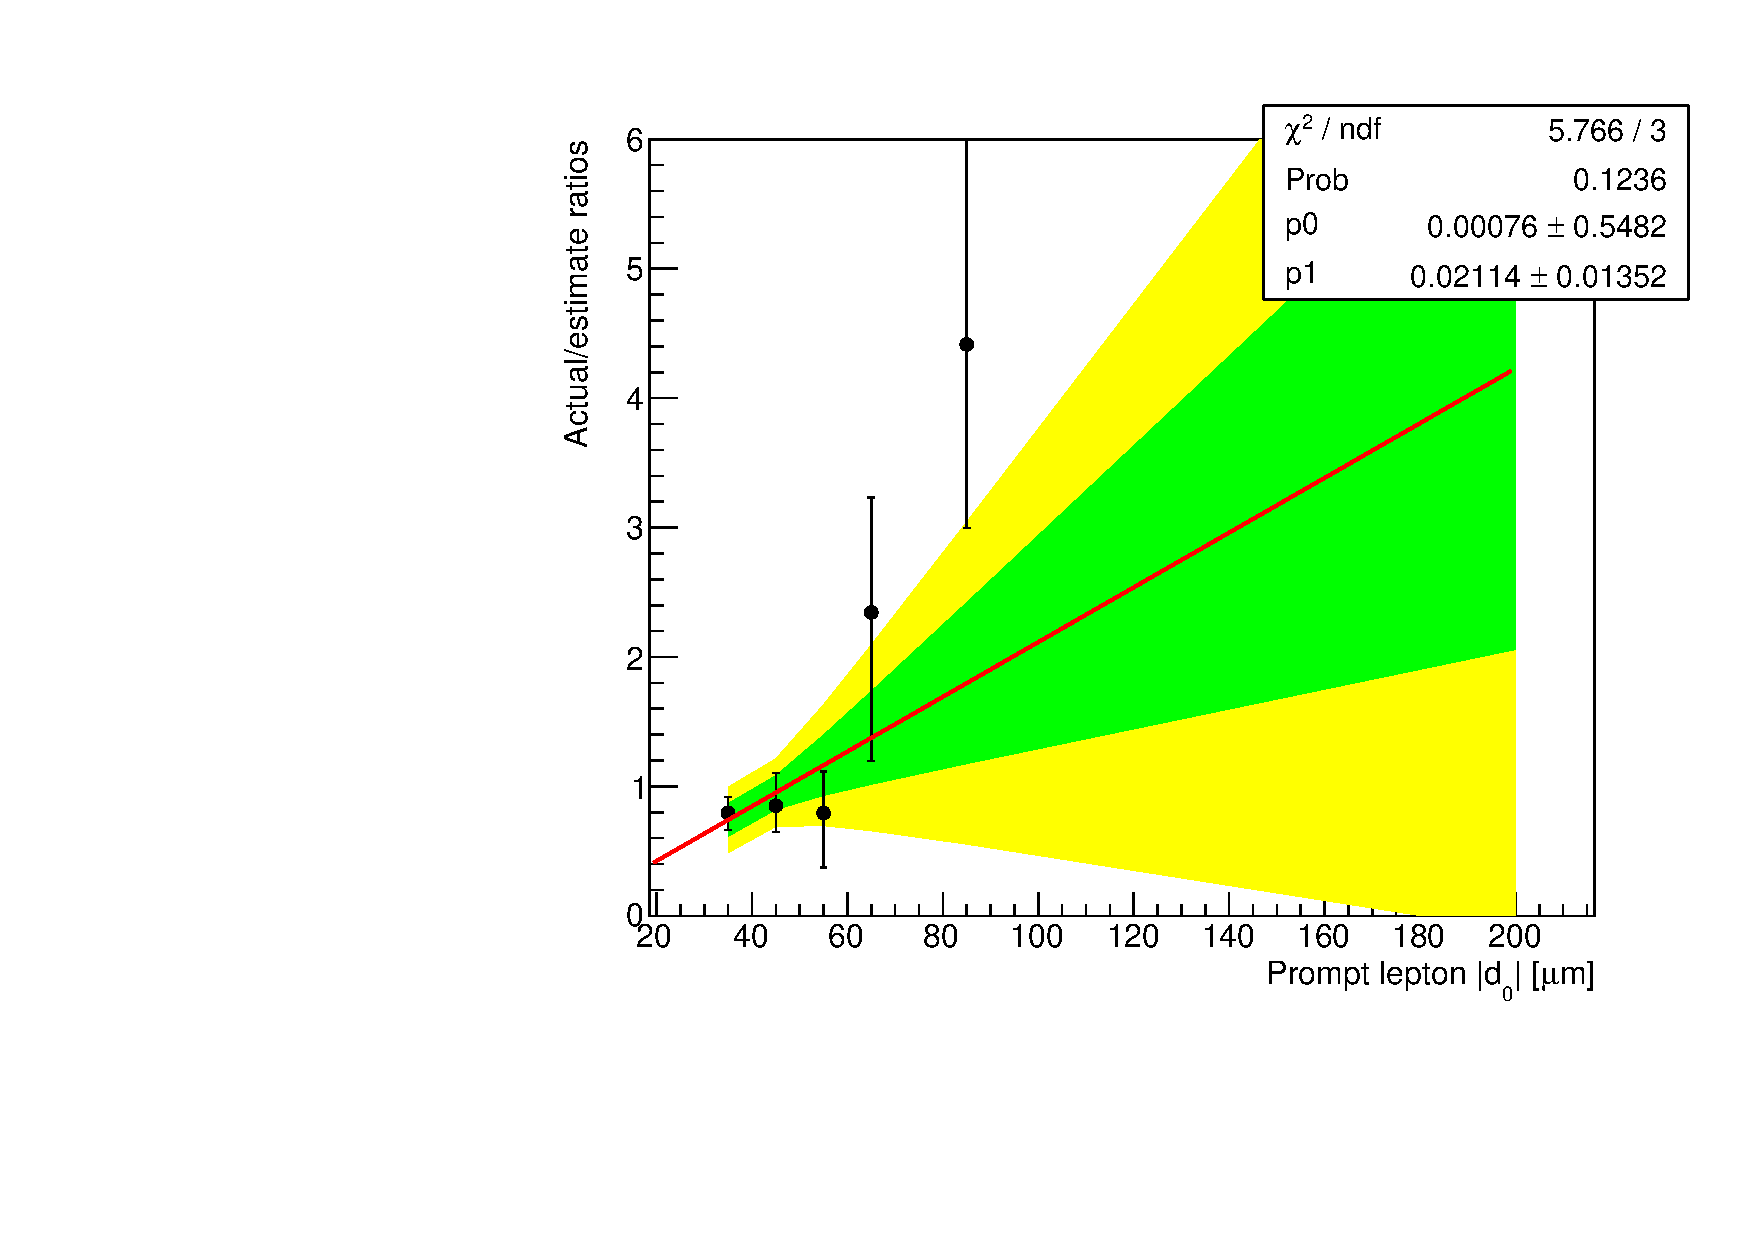
\includegraphics[scale=0.35]{figures/bg/mumu_data_2017_2018_displacedSubleading_ratiosVsPromptD0.pdf}
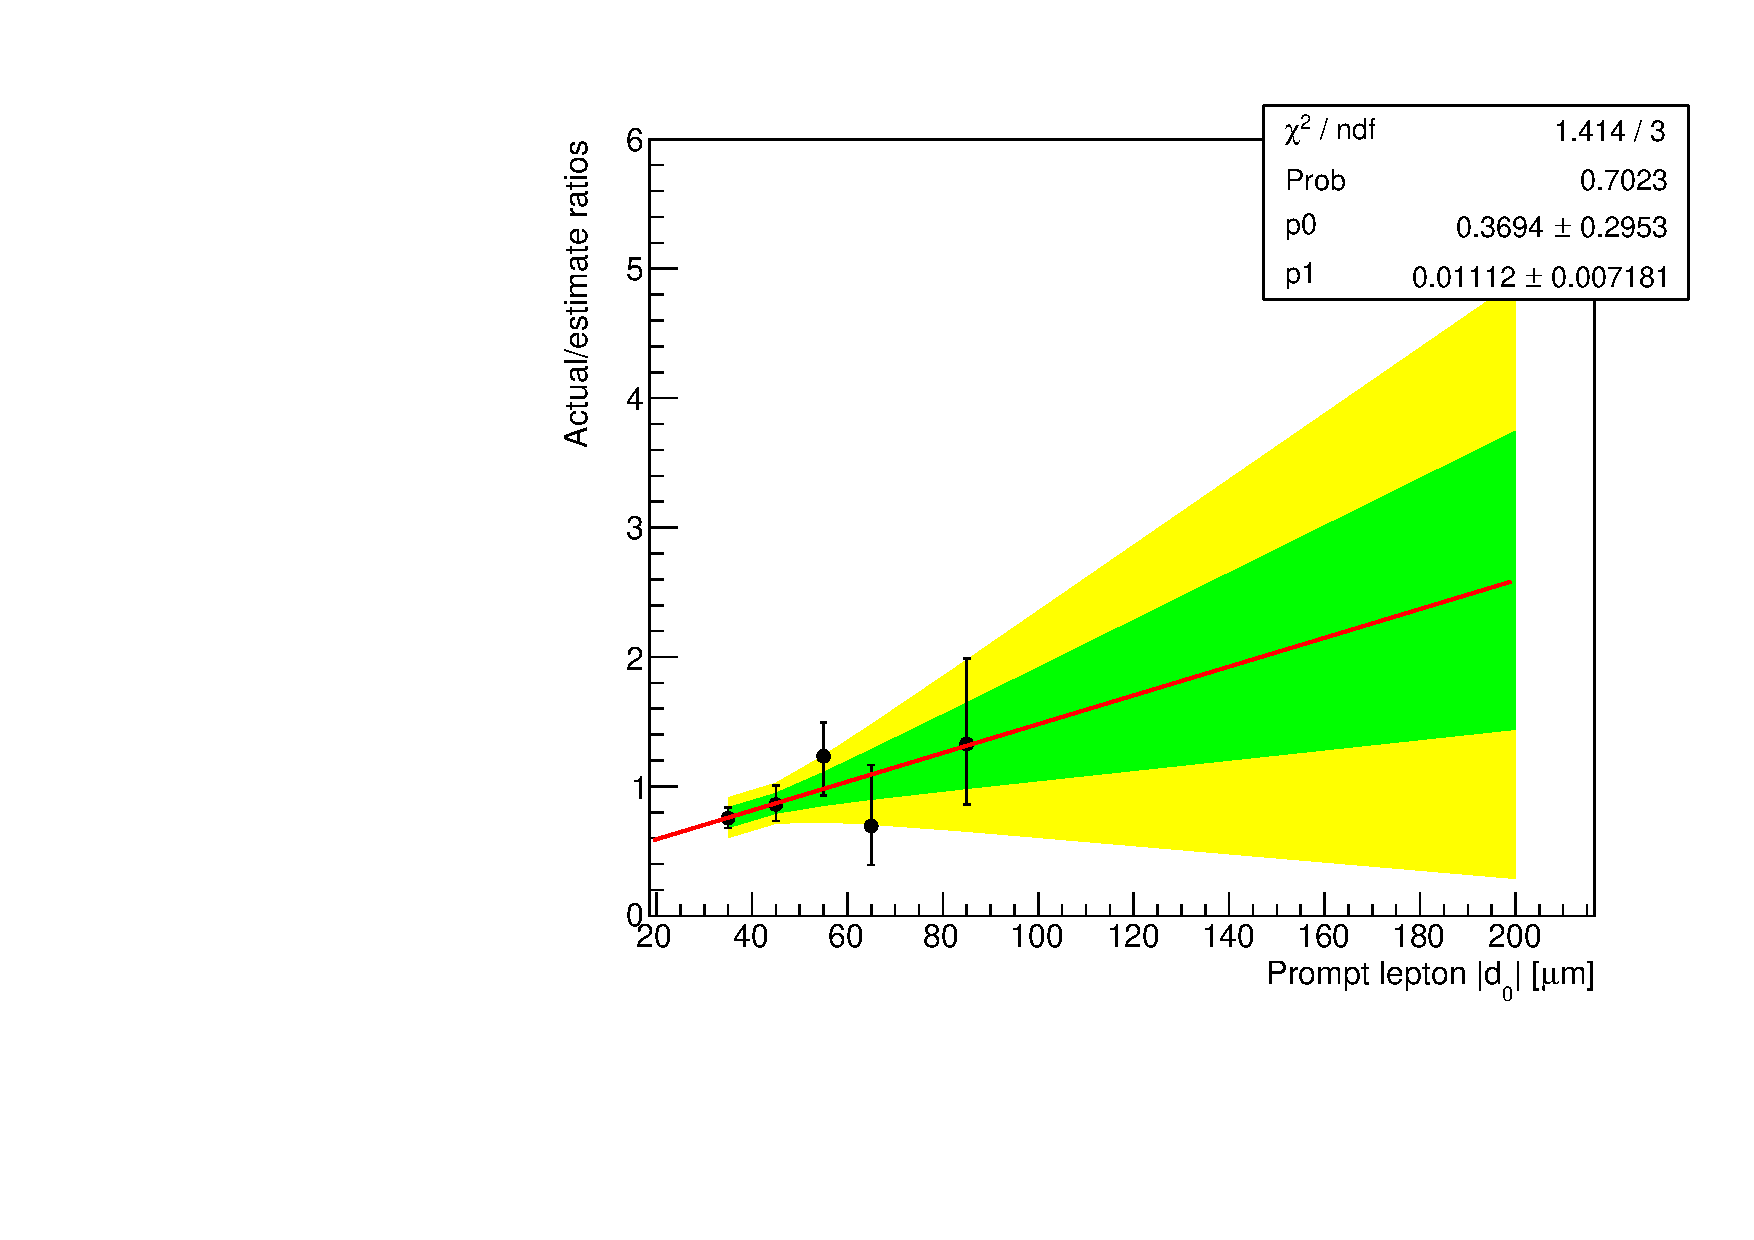
\includegraphics[scale=0.35]{figures/bg/mumu_data_2016_displacedLeading_ratiosVsPromptD0.pdf}
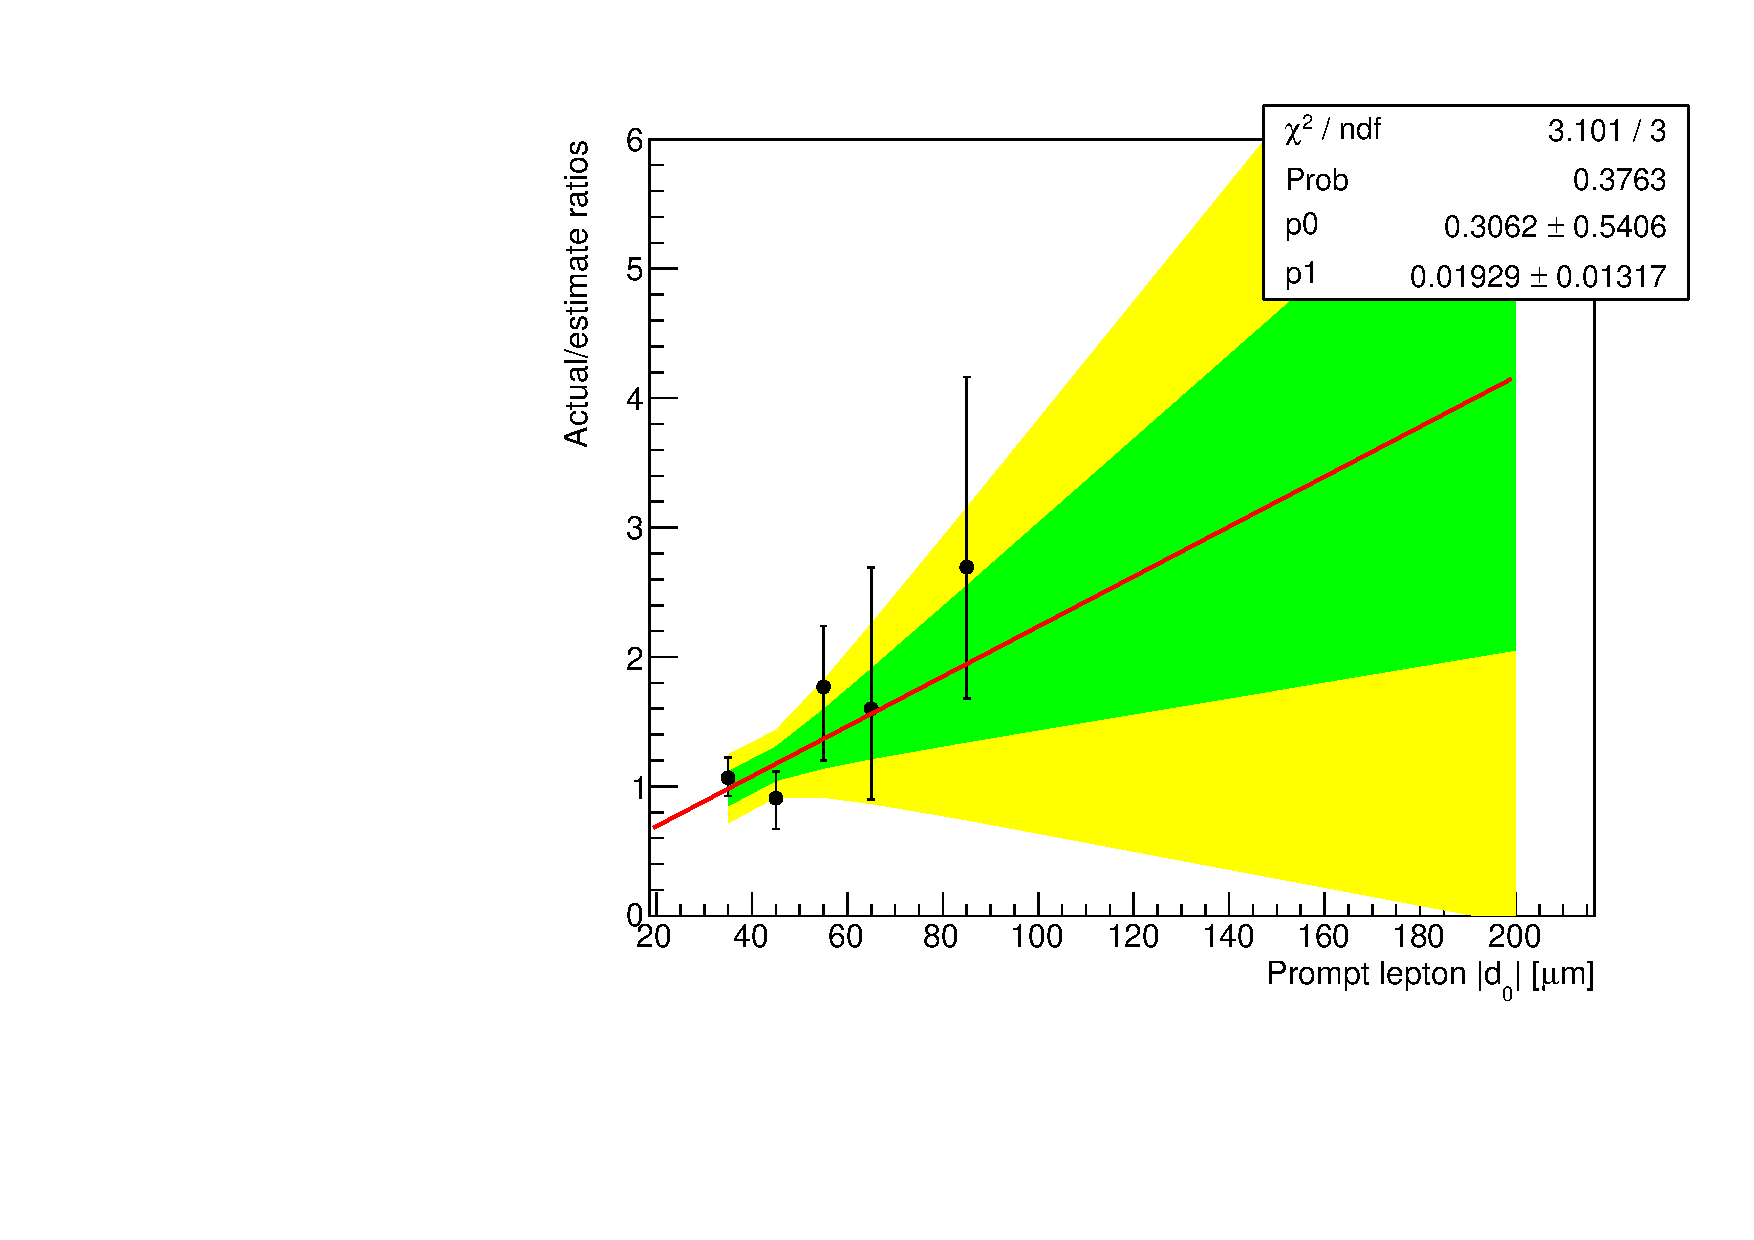
\includegraphics[scale=0.35]{figures/bg/mumu_data_2017_2018_displacedLeading_ratiosVsPromptD0.pdf}
\caption{Background estimation closure tests in data, in the one-prompt (20--100\mum)/one-displaced (100-500\mum) sidebands, in the $\Pgm\Pgm$ channel. The prompt-leading-muon/displaced-subleading-muon sideband is shown in the upper row, and the prompt-subleading-muon/displaced-leading-muon sideband is shown in the lower row. The plots on the left show the results for 2016 data, and the plots on the right are for combined 2017 and 2018 data. The plots show the ratio of the actual to the estimated number of events as a function of the prompt lepton \ad. The data are fitted with a straight line, where the slope and y-intercept are allowed to vary. The $1\sigma$ and $2\sigma$ confidence intervals are shown in the green and yellow bands, respectively.}\fxnote{update to d0a, d0b or B, C language}
\label{100to500um_fits_mumu}
\end{figure}

If the average extrapolated ratio is $>1.0$, we take the central value as a multiplicative correction to the background estimate and the uncertainty in the average as a systematic uncertainty in the background estimate. In this case, we also vary the \SI{200}{\um} extrapolation point by $\pm\SI{50}{\um}$ (the approximate width of the peak in the tau lepton contribution as a function of \ad). We apply the difference from this variation in extrapolation point as an additional systematic uncertainty in the background estimate. If the average is $\leq 1.0$, we set the correction equal to $1.0$ and use the uncertainty in the average as a symmetric systematic uncertainty about $1.0$. Table~\ref{100to500um_estimates} shows the resulting correction factors along with the uncorrected and corrected SR I background estimate.

\begin{table}
\renewcommand{\arraystretch}{1.2}
\noindent \centering{}
\topcaption{The correction factors and the uncorrected and corrected background estimates in SR I . The correction factor uncertainties include both the uncertainty in the average and the additional uncertainty obtained from varying the fit extrapolation point. The total uncertainty (statistical plus systematic) is given for the corrected background estimates.}
\label{100to500um_estimates}
\begin{tabular}{llll}
\hline
  & Correction factor & Uncorrected estimate & Corrected estimate\\
  \hline\\[-2.4ex]
2016 $\Pe\Pgm$       & $1.0^{+1.3}_{-1.0}$    & $4.21^{+0.38}_{-0.40}$  & $4.2^{+5.4}_{-4.2}$\\[0.5ex]
2017+2018 $\Pe\Pgm$  & $3.0\pm1.0$            & $12.53^{+0.64}_{-0.61}$ & $38\pm13$\\[0.5ex]
2016 $\Pe\Pe$        & $1.00\pm0.60$          & $18.30^{+0.94}_{-0.91}$ & $18\pm11$\\[0.5ex]
2017+2018 $\Pe\Pe$   & $1.51^{+0.43}_{-0.42}$ & $41.6\pm1.3$            & $63^{+18}_{-17}$\\[0.5ex]
2016 $\Pgm\Pgm$      & $2.5\pm1.0$            & $3.07\pm0.08$           & $7.7\pm3.1$\\[0.5ex]
2017+2018 $\Pgm\Pgm$ & $4.2\pm1.8$            & $1.00\pm0.04$           & $4.2\pm1.8$\\[0.5ex]
\hline
\end{tabular}
\end{table}

\subsubsection{\SI{500}{\um}--\SI{10}{\cm} systematic uncertainty}
In the \SI{500}{\um}--\SI{10}{\cm} region, we derive a systematic uncertainty in the background estimate from the data closure tests shown in Section~\ref{cr_closure_tests}. We take the largest deviation from \num{1.0} that occurs in the ratio of the actual to the estimated number of events plus its uncertainty, in either of the two closure tests that correspond to a given SR, as a systematic uncertainty. This is a conservative approach that produces a large systematic uncertainty in the small background yields that we predict in these regions. Table \ref{500umto10cm_estimates} shows the systematic uncertainty and the predicted number of events in SRs II, III, and IV.

\begin{table}[ht] 
\noindent \centering{}
\topcaption{The systematic uncertainty and the background estimates in SRs II, III, and IV. The total uncertainty (statistical plus systematic) is given for each estimate.}
\label{500umto10cm_estimates}
\begin{tabular}{lllll}
\hline
  & Systematic uncertainty & SR II & SR III & SR IV\\
  \hline\\[-2.4ex]
2016 $\Pe\Pgm$       & 98\%  & $0.15\pm0.15$           & $0.09^{+0.12}_{-0.09}$ & $0.003^{+0.004}_{-0.003}$\\[0.5ex]
2017+2018 $\Pe\Pgm$  & 106\% & $0.71^{+0.76}_{-0.71}$  & $0.23^{+0.27}_{-0.23}$ & $0.01^{+0.02}_{-0.01}$\\[0.5ex]
2016 $\Pe\Pe$        & 199\% & $0.51^{+1.02}_{-0.51}$  & $0.43^{+0.85}_{-0.43}$ & $0.01^{+0.02}_{-0.01}$\\[0.5ex]
2017+2018 $\Pe\Pe$   & 37\%  & $3.6\pm1.4$             & $2.8\pm1.1$            & $0.24^{+0.10}_{-0.09}$\\[0.5ex]
2016 $\Pgm\Pgm$      & 64\%  & $0.17\pm0.11$           & $0.19\pm0.12$          & $0.01\pm0.01$\\[0.5ex]
2017+2018 $\Pgm\Pgm$ & 140\% & $0.14^{+0.19}_{-0.14}$  & $0.08^{+0.12}_{-0.08}$ & $0.01^{+0.02}_{-0.01}$\\[0.5ex]
\hline
\end{tabular}
\end{table}

\subsection{Testing full background estimation procedure}

Having defined the full background estimation procedure and seen that the \ada-\adb correlation observed in data is also present in simulated background events, we now perform a final closure test of the full background estimation method using simulated background events in SRs I--IV.

Table~\ref{sr_closure_tests} shows the estimated and actual number of simulated background events in SRs I--IV. The listed estimates include all corrections and statistical and systematic uncertainties as discussed in \ref{abcd_correction}. The uncertainties in the actual values are purely statistical. The general agreement between estimated and actual yields leads us to conclude that the background estimation procedure is valid and the assigned systematic uncertainties are sufficient to cover any potential sources of nonclosure that we have not explicitly considered.

\begin{table}
\renewcommand{\arraystretch}{1.3}
\noindent \centering{}
\topcaption{Closure test results in background simulation in the SRs with all background estimate corrections and uncertainties applied. The estimated number of events, the actual number of events, and their total uncertainties (statistical plus systematic) are given. In cases where the actual number of events is zero, the uncertainty is given by the product of the average background simulation event weight and the upper bound of the 68\% Poisson interval given by a single observation of zero events.}
\label{sr_closure_tests}
\begin{tabular}{l|llll}
  & SR I & SR II & SR III & SR IV\\
\hline
2016 $\Pe\Pgm$ estimated       & $7.4^{+4.8}_{-4.2}$    & $0.07\pm0.07$          & $0.096^{+0.105}_{-0.096}$ & $0.001\pm0.001$\\
2016 $\Pe\Pgm$ actual          & $5.0^{+1.5}_{-1.2}$    & $0.07^{+0.09}_{-0.05}$ & $0.005^{+0.011}_{-0.004}$ & $0.000^{+0.037}_{-0.000}$\\
\hline
2017+2018 $\Pe\Pgm$ estimated  & $13.5\pm6.4$           & $0.37^{+0.40}_{-0.37}$ & $0.34^{+0.36}_{-0.34}$    & $0.02\pm0.02$\\
2017+2018 $\Pe\Pgm$ actual     & $19.1^{+11.4}_{-7.6}$  & $0.52^{+0.41}_{-0.25}$ & $0.00^{+0.24}_{-0.00}$    & $0.00^{+0.24}_{-0.00}$\\
\hline
2016 $\Pe\Pe$ estimated        & $9.3\pm5.0$            & $0.12^{+0.23}_{-0.12}$ & $0.14^{+0.28}_{-0.14}$    & $0.002^{+0.004}_{-0.002}$\\
2016 $\Pe\Pe$ actual           & $13.4^{+3.4}_{-2.8}$   & $0.15^{+0.19}_{-0.09}$ & $1.03^{+1.36}_{-0.67}$    & $0.000^{+0.550}_{-0.000}$\\
\hline
2017+2018 $\Pe\Pe$ estimated   & $18\pm11$              & $0.59^{+0.27}_{-0.26}$ & $0.45^{+0.21}_{-0.20}$    & $0.02\pm0.01$\\
2017+2018 $\Pe\Pe$ actual      & $8.2^{+6.5}_{-3.9}$    & $0.17^{+0.23}_{-0.11}$ & $0.00^{+0.17}_{-0.00}$    & $0.00^{+0.17}_{-0.00}$\\
\hline
2016 $\Pgm\Pgm$ estimated      & $1.3\pm0.6$            & $0.04\pm0.04$          & $0.03\pm0.03$             & $0.002\pm0.002$\\
2016 $\Pgm\Pgm$ actual         & $3.3^{+1.8}_{-1.2}$    & $0.11^{+0.14}_{-0.07}$ & $0.06^{+0.14}_{-0.05}$    & $0.000^{+0.110}_{-0.000}$\\
\hline
2017+2018 $\Pgm\Pgm$ estimated & $2.7\pm1.4$            & $0.04\pm0.04$          & $0.02\pm0.02$             & $0.002\pm0.002$\\
2017+2018 $\Pgm\Pgm$ actual    & $7.1^{+6.9}_{-3.8}$    & $0.00^{+0.15}_{-0.00}$ & $0.00^{+0.15}_{-0.00}$    & $0.078^{+0.179}_{-0.064}$\\
\hline
\end{tabular}
\end{table}

\subsection{Additional background checks}
\label{additional_bg_checks}
We perform a few additional studies to check for other potential sources of background. We find that their SR contributions are either negligible or already covered by the background estimation method described above.

\subsubsection{Material interactions}
In order to further study the material interactions, we invert the preselection criterion that rejects good vertices in the material. In data, we find seven events, across all channels and years, that pass the preselection with this inverted criterion. As shown in Table~\ref{material_interaction_evts}, three of these events are in the prompt control region and four are in region B or region C. The lepton vertices in these events coincide with the material as we expect: two are in the beampipe, one is in the pixel detector inner shield, and four are in the first layer of the pixel detector. Even with the material interaction veto inverted, we find no SR events resulting from material interactions and therefore conclude that material interactions are not a significant background after the full selection is applied.

\begin{table}[ht]
\noindent \centering{}
\topcaption{Some properties of the seven events found in data with the material interactions selection inverted.}
\label{material_interaction_evts}
\begin{tabular}{lll}
\hline
Channel, year & \ada, \adb [\mum] & vertex position (x, y, z) [\cm]\\
\hline
$\Pe\Pgm$ 2017C  & -14,   -10 (A) & (-2.5, 1.4, 6.8) (BPIX L1)\\
$\Pe\Pgm$ 2018D  &  46,   -14 (A) & (0.9, 2.1, 0.1) (beampipe)\\
$\Pe\Pe$ 2018D   & 198,   -34 (B) & (-1.9, 0.5, 2.7) (beampipe)\\
$\Pgm\Pgm$ 2016G & 407,    -8 (B) & (-1.4, 4.0, 6.3) (BPIX L1)\\
$\Pgm\Pgm$ 2016G & -17, -2215 (C) & (-2.6, 3.1, 6.6) (BPIX L1)\\
$\Pgm\Pgm$ 2016H &   2,     0 (A) & (-1.6, -3.5, 12) (BPIX inner shield)\\
$\Pgm\Pgm$ 2017F & 522,   -13 (B) & (-1.1, -3.0, -7.5) (BPIX L1)\\
\hline
\end{tabular}
\end{table}

\subsubsection{Cosmic-ray muons}
To estimate the SR contribution of cosmic-ray muons, we perform a study in which we invert the $\Delta t$ and $\cos{\alpha}$ criteria in the \Pgm\Pgm\ preselection and check how many events are in the SRs. We find three data events with the criteria inverted (one event per year, all in SR IV). Next, we use \texttt{NoBPTX} data, which is dominated by cosmic-ray muon events, to estimate the efficiency for cosmic-ray muons to pass the $\Delta t$ and $\cos{(\alpha)}$ criteria after passing the rest of the \Pgm\Pgm\ preselection criteria. While \num{3736} \texttt{NoBPTX} data events pass the preselection criteria with the $\Delta t$ and $\cos{(\alpha)}$ criteria removed, zero \texttt{NoBPTX} data events pass the full preselection. To conservatively estimate the efficiency, we fluctuate the number of passing events up to 1 and find an efficiency of $1/3736$. We therefore find the approximate upper bound on the SR contribution of cosmic ray muons to be $3\times\frac{1}{3736}=0.0008$, which is negligible compared to the background estimation in each SR.

\subsubsection{Heavy-flavor mesons}
We perform two studies to estimate an upper limit on the SR contribution of leptons from heavy-flavor mesons. First, we estimate SR yields with a simple ABCD method in 2018 \Pgm\Pgm\ preselection data while additionally requiring at least one medium CSVv2 \PQb-tagged jet~\cite{bjet_identification}. The test is performed in the \Pgm\Pgm\ channel because it contains the smallest relative SR contribution from mismeasurements and should therefore be most sensitive to heavy flavor. As shown in Table~\ref{abcd_hf_data}, the background estimates are about an order of magnitude smaller than when no \PQb-tagged jet is required in our usual preselection.

\begin{table}
\renewcommand{\arraystretch}{1.3}
\noindent \centering{}
\topcaption{Background estimates in data while applying the 2018 $\Pgm\Pgm$ preselection and the additional requirement of at least one \PQb-tagged jet. The estimates with at least one \PQb-tagged jet are about an order of magnitude below the nominal prediction.}
\label{abcd_hf_data}
\begin{tabular}{lllll}
\hline
& SR I & SR II & SR III & SR IV\\
\hline
Preselection (corrected)  & $2.6\pm1.0$   & $0.09^{+0.12}_{-0.09}$    & $0.05^{+0.07}_{-0.05}$    & $0.007^{+0.010}_{-0.007}$\\
Preselection + 1 \PQb jet & $0.19\pm0.03$ & $0.008^{+0.007}_{-0.004}$ & $0.005^{+0.004}_{-0.002}$ & $0.0002^{+0.0002}_{-0.0001}$\\
\hline
\end{tabular}
\end{table}

Next, we look at 2018 data and simulated QCD multijet events that pass the \Pgm\Pgm\ preselection with the isolation criterion inverted. These samples are dominated by muons from B meson decays, and the QCD simulation describes the data well in the region outside of the \cPZ\ boson peak, as shown in Fig.~\ref{mumu_inv_mass_inverted_iso}. We use this QCD multijet sample to test the heavy-flavor background in two ways. First, we perform a simple ABCD estimate in the simulated QCD multijet events to check for \ada-\adb correlation. As shown in Table~\ref{abcd_hf_mc}, we find no evidence of correlation, which indicates that the background estimation already accounts for the heavy-flavor background. Second, we estimate the approximate heavy-flavor background in the SRs by taking the ratio of SR to prompt control region events in QCD multijet simulation from the anti-isolated region and the normalization from the number of simulated QCD multijet events that pass the \Pgm\Pgm\ preselection. Using this approach, we estimate that the heavy-flavor background to be $0.06^{+0.13}_{-0.05}$ events in SR I and $0.0015^{+0.0034}_{-0.0012}$ events in SR IV, which is small relative to the nominal prediction shown in the first row of Table~\ref{abcd_hf_data}.

\begin{figure}
\centering
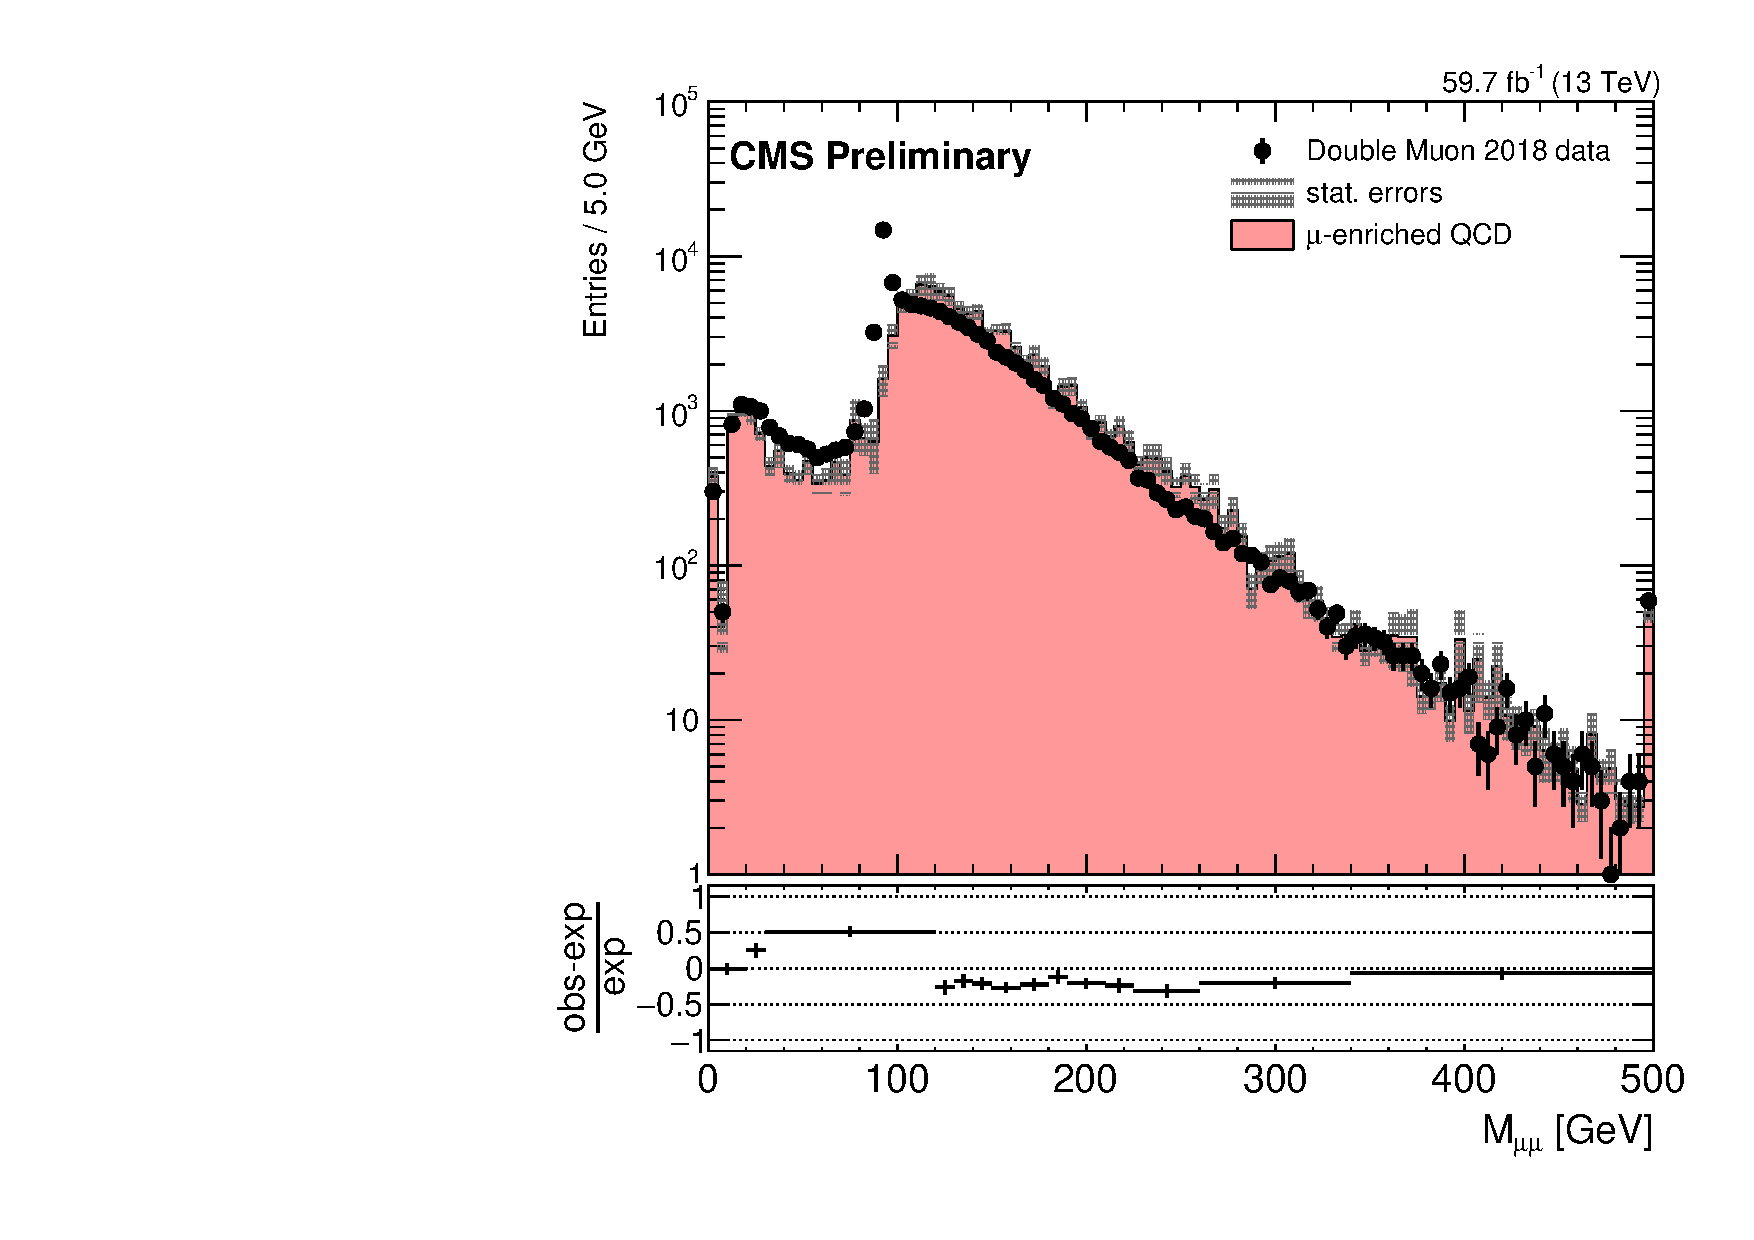
\includegraphics[width=0.5\textwidth]{figures/bg/mumuInvMass_qcd_vs_data.pdf}
\caption{The di-muon invariant mass distribution in data and QCD multijet simulation events that pass the 2018 $\Pgm\Pgm$ preselection with the muon isolation criterion inverted.}
\label{mumu_inv_mass_inverted_iso}
\end{figure}
\begin{table}[ht]
\renewcommand{\arraystretch}{1.3}
\noindent \centering{}
\topcaption{A closure test of the ABCD method in 2018 QCD simulation in the $\Pgm\Pgm$ channel with the muon isolation criterion inverted. The estimates from the ABCD method, the actual yields in simulation, and the ratios of the actual to the estimated yields are shown.}
\label{abcd_hf_mc}
\begin{tabular}{llll}
\hline
Region & Estimated yield & Actual yield & Ratio of actual to estimate\\
\hline
SR I	& $9500\pm1100$	        & $11000\pm1000$	    & $1.2\pm0.2$\\
SR II	& $1740^{+310}_{-280}$	& $2200^{+330}_{-290}$	& $1.3\pm0.3$\\
SR III	& $1450^{+280}_{-240}$	& $1500^{+180}_{-160}$	& $1.0\pm0.2$\\
SR IV	& $265^{+62}_{-54}$	    & $268^{+61}_{-50}$	    & $1.0\pm0.3$\\
\hline
\end{tabular}
\end{table}

We therefore conclude that the heavy-flavor SR contribution is small and already accounted for in our background estimates.

\subsubsection{Low-mass SM hadrons}
To estimate an upper limit on the SR contribution of leptons from decays of low-mass SM hadrons, we examine 2018 data and QCD multijet simulation in the \Pgm\Pgm\ channel with both the muon isolation and the $\DR$ requirements inverted. As shown in Fig.~\ref{mumu_inv_mass_inverted_iso_lo}, this region is dominated low-mass \Pgm\Pgm\ pairs, with clear J/$\psi$, $\psi^\prime$, and $\Upsilon$ mass peaks. Many of these leptons are displaced, especially those in the J/$\psi$ mass range. To estimate the fraction of such leptons that will be displaced, we take the ratio of SR to prompt control region events of SM hadrons that decay to leptons from data in this region.

\begin{figure}
\centering
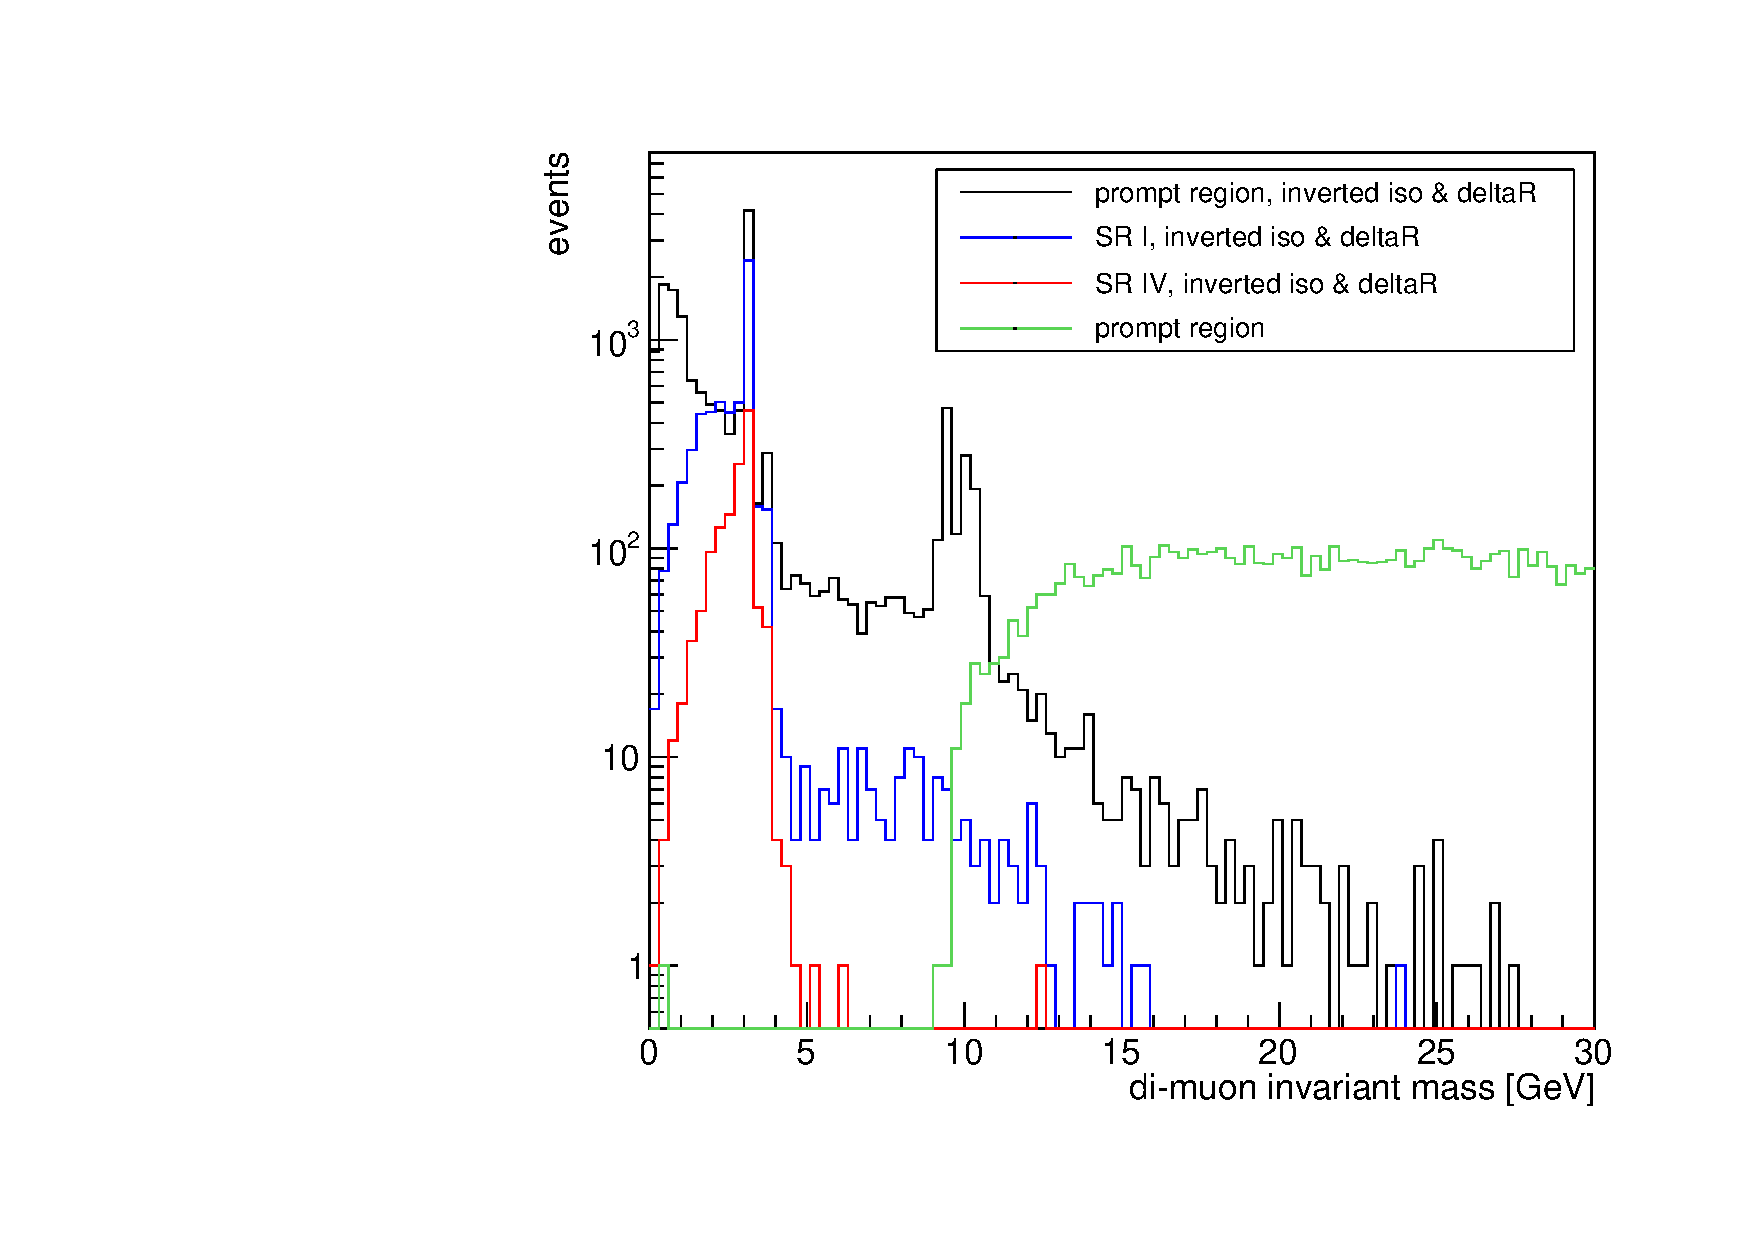
\includegraphics[width=0.6\textwidth]{figures/bg/mumuInvMass_comparison.pdf}
\caption{The dimuon invariant mass distribution in 2018 data in the $\Pgm\Pgm$ channel, in the prompt control region (black), SR I (blue), SR IV (red), with the muon isolation and di-muon $\DR$ criteria inverted. The equivalent distribution from the prompt control region is also shown in green.}
\label{mumu_inv_mass_inverted_iso_lo}
\end{figure}

Even though the inverted-isolation region is dominated by low-mass muon pairs, the only QCD multijet simulation event that survives the 2018 \Pgm\Pgm\ preselection has a di-muon invariant mass of approximately 300\GeV. Furthermore, the muons are not near each other in the $\eta$-$\phi$ plane ($\DR\approx3$), which is inconsistent with the low-mass SM hadron events that dominate the region with the inverted isolation and $\DR$ criteria. To find a normalization from which to estimate the low-mass SM hadron SR contribution, we therefore turn to the inverted-isolation sample used above in the heavy-flavor meson cross check. In this sample, the ratio of events with $\DR<0.5$ to events with $2.8<\DR<3.2$ is about $0.1$. We find $0.2$ QCD multijet simulated events that pass the nominal preselection, and so we estimate that of the events passing the 2018 \Pgm\Pgm\ preselection, about $0.02$ contain pairs of muons produced in low-mass SM hadron decays. We estimate the SR contributions using this preselection normalization and the ratio of SR to prompt control region events from the sample of SM hadrons that decay to leptons in data. We find this contribution is less than $0.006^{+0.013}_{-0.005}$ events in SR I and less than $0.001^{+0.002}_{-0.001}$ events in SR IV, which, if compared with the nominal prediction shown in the first row of Table~\ref{mumu_inv_mass_inverted_iso}, are respectively negligible and easily covered by the \SI{140}{\percent} systematic uncertainty already applied to the background prediction in this region.

\pagebreak